\vspace{-4pt}
\section{Analysis of Design Constraints - A Case Study}\label{sec:w_and_r}

In this section, we study the effect of various schemes on cross-point
size and reliability in detail by using our mathematical model. The
constraints on array size, energy consumption and area overhead are
analyzed in the worst cases scenario. The results of this study will be a
useful guide in designing a cross-point array.

\vspace{-10pt}
\subsection{Overview}
%As shown in Figure~\ref{fig:modeling}, i
In order to write or read a cross-point array, proper voltages should be
applied across the ReRAM cell. Although the goal of a read operation is
different from a write operations, both of them are realized by fully
biasing the selected wordlines/bitlines and floating (or half biasing)
unselected wordlines/bitlines. Thus, the coefficient matrix $A$ and the
constant vector $C$ are very similar for both. In addition, their energy
consumption and area overhead will also have a similar trend. Therefore,
in this section, we first study the write operation comprehensively. After
that, for read operation, we mainly focus on the read margin analysis
since it is unique to reads.
%can be very useful to guide the design of the cross-point array.
%Also, we assumes that the in the case of worst scenario, the ReRAM cells at the selected wordline, th
%Since it is impossible to consider all of the data pattern stored in the array,

Table~\ref{table:parameter} shows the circuit parameters of our baseline
50nm design. The data is derived from the recently published studies on
ReRAM~\cite{?????,memristor:Cong}. We study reliability, energy
consumption, and area overheads for four different write schemes, and
discuss the sensitivities of these schemes to the data pattern of HRS and
LRS ReRAM cells and cell non-linearity.

\begin{table}[!b]
  \centering
  \scriptsize
    \scriptsize
  \caption{Parameters of the baseline Cross-Point Array}\label{table:parameter}
  \vspace{-5pt}
%  \begin{tabular}{|cccccp{3.5cm}|}
  \begin{tabular}{c|c|c}
    \hline    \hline
    % after \\: \hline or \cline{col1-col2} \cline{col3-col4} ...
    \textbf{Metric} & \textbf{Description} & \textbf{Typical Values (Range)} \\
    \hline
    \textbf{$S_{cell}$} & Cell Size & \textbf{$4F^2$} \\
    \textbf{$R_l$} &  Interconnection Resistance&\textbf{$0.65\Omega$} \\
    \textbf{$V_{RESET}$} & Threshold voltage for RESET&\textbf{$2.0V$} \\
    \textbf{$V_{SET}$} & Threshold voltage for SET&\textbf{$-2.0V$} \\
    \textbf{$V_{READ}$} & Read Voltage of Cell&\textbf{$0.5V$} \\
    \textbf{$I_{on}$} & Write Current for LRS Cell &\textbf{$40uA$~~($20\sim200uA$)} \\
    \textbf{$V_{W}(R)$} & Wordline Voltage during Read &\textbf{$0.4V$} \\
    \textbf{$V_{W}(W)$} & Wordline Voltage during Write  &\textbf{$\pm2V$} \\
    \textbf{$V_{W}(H)$} & Half Selected wordline Voltage &\textbf{$1V$} \\
    \textbf{$V_{B}(R)$} & Bitline Voltage during Read  &\textbf{$0V$} \\
    \textbf{$V_{B}(W)$} & Bitline Voltage during Write  &\textbf{$0V$} \\
    \textbf{$V_{B}(H)$} & Half Selected bitline Voltage &\textbf{$1V$} \\
    \textbf{$K_r$} & Nonlinearity of ReRAM Cell &\textbf{$5$~~($2\sim40$)} \\
    \textbf{$M,N$} & Number of wordlines/bitlines &\textbf{$512$~~($8\sim1024$)} \\
    \hline
  \end{tabular}
  \vspace{-10pt}
\end{table}

\subsection{Write Operation}
To write a ReRAM cell, an external voltage is applied across the cell for
a certain duration. Intuitively, there are four possible schemes for the
write operation:
\begin{enumerate}
  \item According to the location of a selected cell, activate one
      wordline and one bitline and leave all of other lines floating
      (FWFB shemes).
  \item Activate the selected wordline and bitline. Leave all the
      unselected wordlines floating and half bias the unselected
      bitlines (FWHB shemes).
  \item In contrast to the scheme 2), activate the selected wordline
      and bitline. Leave all the unselected bitlines floating and half
      bias the unselected wold lines (HWFB shemes).
  \item Activate the selected wordline and bitline. Then half bias all
      other wordlines and bitlines (HWHB shemes).
\end{enumerate}
However,the FWFB scheme has inherent problem that may result in severe
write disturbance~\cite{??}. Therefore, in the following discussion, we
only compare the results of FWHB, HWFB and HWHB schemes. For each of these
three schemes, we can either write several cells at one wordline at the
same time or only write one bit per access and distribute the write
operation to several arrays. In the following discussion, we start from
one bit per access write operation, then the results of one wordline per
access method are discussed.

%Since several potential read/write schemes can be used to program a memory array, it is difficult to identify the ideal scheme that meets the design constraints in terms of area, energy, and reliability.
%However, the FWFB scheme has inherent problem that may result in severe
%write disturbance. For example, for writing a ReRAM cell located at the
%cross point of the $i^{nd}$ wordline and the $j^{nd}$ bitline in a $M
%\times N$ matrix ($M>N$), the worst case voltage drop of unselected cells
%appears when all of the ReRAM cells at the selected bitline are in the
%HRS, while all of the other cells are in the LRS. In this case, the
%voltage drop across the selected cell almost has the same magnitude as the
%unselected cell at the same bitline, resulting the write disturbance to
%all of the unselected cells at the selected bitline. Actually, the worst
%case voltage drop of the unselected cell can be calculated as:
%\begin{equation}\label{worst_FWFB}
%V_{worst}=V_{select} \cdot [1-\frac{1}{M+(N-1)R_{off}/R_{on}}].
%\end{equation}
%Considering that the reported On-OFF resistance ratio of ReRAM cell is
%always $>50$
%~\cite{ReRAM_IEDM2010_Ho,ReRAM_IEDM2010_Chien,ReRAM_IEDM2010_Lee_Diode,ReRAM_IEDM2010_Lee_Evidence,ReRAM_ISSCC2011_Sheu,ReRAM_ISSCC2011_Otsuka},
%, the worst case voltage drop at the unselected cell is larger than $98\%$
%of the voltage at the selected cell, making it is impossible to build a
%reliable cross-point structure ReRAM with the FWFB scheme. Therefore, in
%the following discussion, we only compare the results of FWHB, HWFB and
%HWHB schemes. For each of these three schemes, we can either write several
%cells at one wordline at the same time or only write one bit per access
%and distribute the write operation to several arrays. In the following
%discussion, we start from one bit per access write operation, then the
%results of one wordline per access method are discussed.

%Since reliability, energy consumption, and area overheads for these
%schemes are different, we address these problems separately and finally
%combine all constraints to provide design guidelines for write operations.


\vspace{6pt} \emph{Reliable Write Operation.} \vspace{6pt}

Write reliability is a serious concern in cross-point arrays. In an ideal
condition, the resistance of wires and the sneak currents in unselected
cells are negligible. In such a scenario, all the write schemes discussed
above will make sure that the write voltage $V_W(W)-V_B(W)$ is fully
applied across the specified cell. However, in reality, both wire
resistance and sneak current are non-trivial. Hence, the operation of
cross-point array will vary based on the data pattern stored in ReRAM
cells. A write is considered reliable if it modifies the content of the
selected cells to the new value without disturbing other unselected cells.
%A reliable write operation can be defined as: switching the selected cells into required states without disturbing the states of unselected cells.
There are two potential problems with writes: \emph{write failure}, an
unsuccessful write on selected cell, and \emph{write disturbance}, an
undesirable write on unselected cell. It is necessary to ensure that a
write scheme guarantees reliable operation even in the worst case (w.r.t
the location of cells to written and the data pattern stored in the
cross-point array). Otherwise, after several unreliable write operations,
the data stored in the cross-point array will become unpredictable.

%We first use an example to show the problem with FWFB scheme, which may
%result in severe write disturbance. Figure~\ref{fig:FWFR} shows the
%voltage drop across each ReRAM cell of a $64 \times 64$ cross-point array.
%In this example, in order to write the cell at the cross point of the
%$32^{nd}$ wordline and the $32^{nd}$ bitline, the selected wordline and
%bitline are biased at 2V and 0V, respectively. All of the other wordlines
%and bitlines are left floating. The ReRAM cells at the selected bitline are
%in the HRS, while all of the other cells are in the LRS. It is clear that
%the voltage drop across the selected cell ($V_{32,32}$) almost has the
%same magnitude as the unselected cell at the same bitline, resulting the
%write disturbance to all of the unselected cells at the selected bitline.
%Actually, for a $M \times N$ matrix ($M>N$), the worst case voltage drop
%of the unselected cell can be calculated as:
%\begin{equation}\label{worst_FWFB}
%V_{worst}=V_{select} \cdot [1-\frac{1}{M+(N-1)R_{off}/R_{on}}].
%\end{equation}
%
%\begin{figure}[!b]
%\centering
%  % Requires \usepackage{graphicx}
%  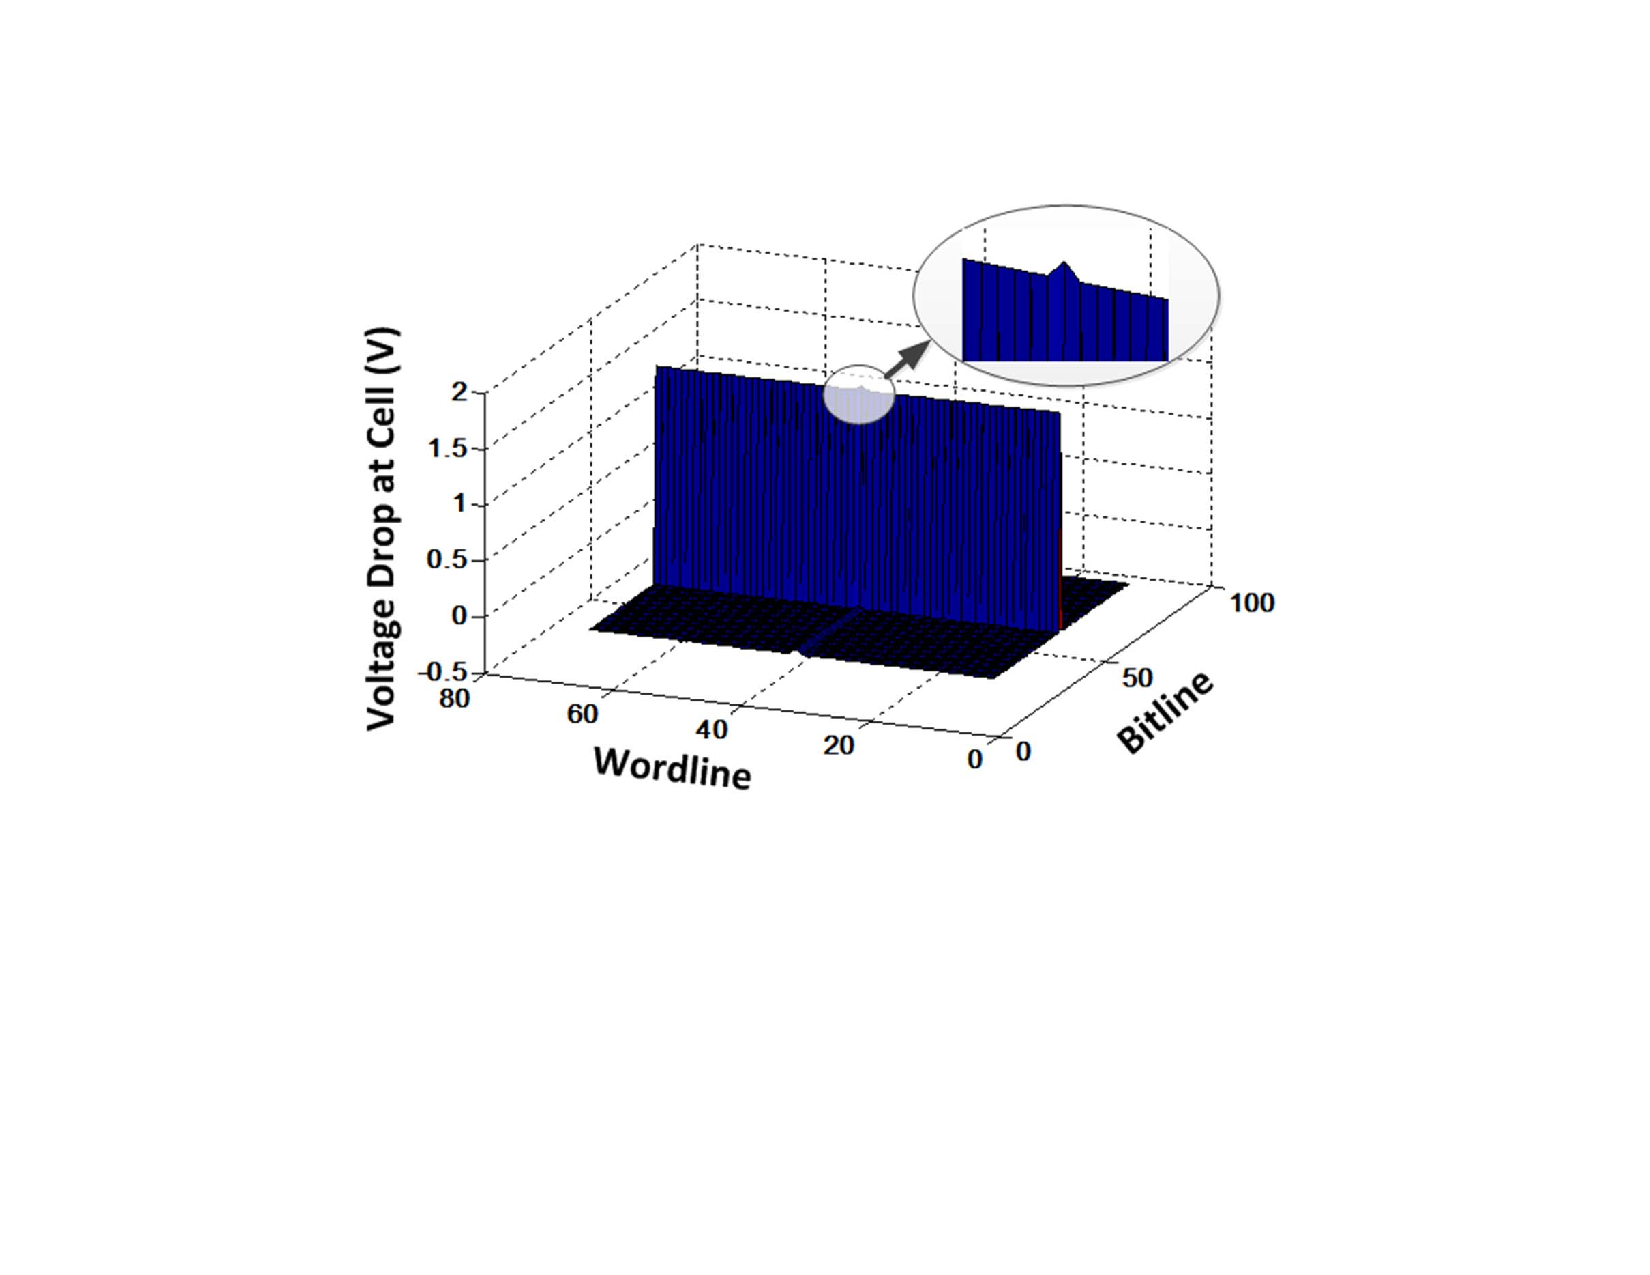
\includegraphics[width=0.4\textwidth]{./figures/FWFB_f.pdf}\\
%  \caption{Write disturbance for FWFB schemes. ( $V_{W32} = 2V$, $V_{B32} = 0V$. $R_{x,32}$ at HRS, others at LRS.) }\label{fig:FWFR}
%\end{figure}
%Considering that the reported On-OFF resistance ratio of
%ReRAM cell is always $>50$ ~\cite{ReRAM_IEDM2010_Ho,ReRAM_IEDM2010_Chien,ReRAM_IEDM2010_Lee_Diode,ReRAM_IEDM2010_Lee_Evidence,ReRAM_ISSCC2011_Sheu,ReRAM_ISSCC2011_Otsuka},
%, the worst case voltage drop at the unselected cell is larger than $98\%$ of the voltage at the selected cell, making it is impossible to build a reliable cross-point structure ReRAM with the FWFB scheme. Therefore, in the following discussion, we only compare the results of FWHB, HWFB and HWHB schemes. For each of these three schemes, we can either write the cells at one wordline at the same time or only write one bit per access and separate the write operation to several arrays. In the
%following discussion, we start from one bit per access write operation,
%then the results of one wordline per access method are discussed.


%as long all of unselected cells in the activated wordline (or all of unselected cells in the activated bitline) are at HRS and other cells are in LRS, the voltage drop at unselected cells are mainly applied at the HRS cells at the wordline (or bitline).
%The worse case scenario for FWFB write disturbance can be defined as: all of unselected cells in the activated wordline (or all of unselected cells in the activated bitline) are at HRS and other cells are in LRS. In this case, the voltage drop at unselected cells are mainly applied at the HRS cells at the wordline (or bitline).

Write failure typically results from the voltage drop at the interconnect
wires along the wordline and bitline. It has been shown
that~\cite{crossbar_TED_2010}, for one bit per access write operation, the
worst case voltage drop occurs when writing the cell at the cross point of
the $M^{th}$ wordline and the $N^{th}$ bitline with all of the cells in
the array are in LRS. In order to avoid the write failure and successfully
program the selected ReRAM cell, the driven voltage should be boosted to a
higher level, making sure that the voltage across the cell exceeds the
threshold voltage even at the worst case. Figure~\ref{fig:worst_v} shows
the lower bound of the driven voltage for different sizes of cross-point
array. The minimum wordline/bitline voltage increases from 2.01~V for a
$32 \times 32$ array to nearly 7~V for a $1024 \times 1024$ cross-point
array. In addition, for a memory capability, the cross-point array can be
organized with different number of wordlines and bitlines. For example, a
256K bits cross-point array can be implemented either by a $512 \times
512$ array or by a $64 \times 4096$ array. In the latter case, the voltage
drops along the wordline will be much more serious than along the bitline.
Figure~\ref{fig:shape} examines the voltage requirement for different
array organizations with different write schemes. The result shows that
from a reliability point of view, a cross-point array with same numbers of
wordlines and bitlines is the best choice. Furthermore, we also notice
that when the array has the same number of wordlines and bitlines, FWFB,
HWFB and FWHB schemes have the same minimum driven voltage.

%Clearly, the magnitude of the voltage drop increases with the array size and the resistance of interconnect wires.

\begin{figure}%[!hb]
\centering
\hspace{-5pt}
  % Requires \usepackage{graphicx}
  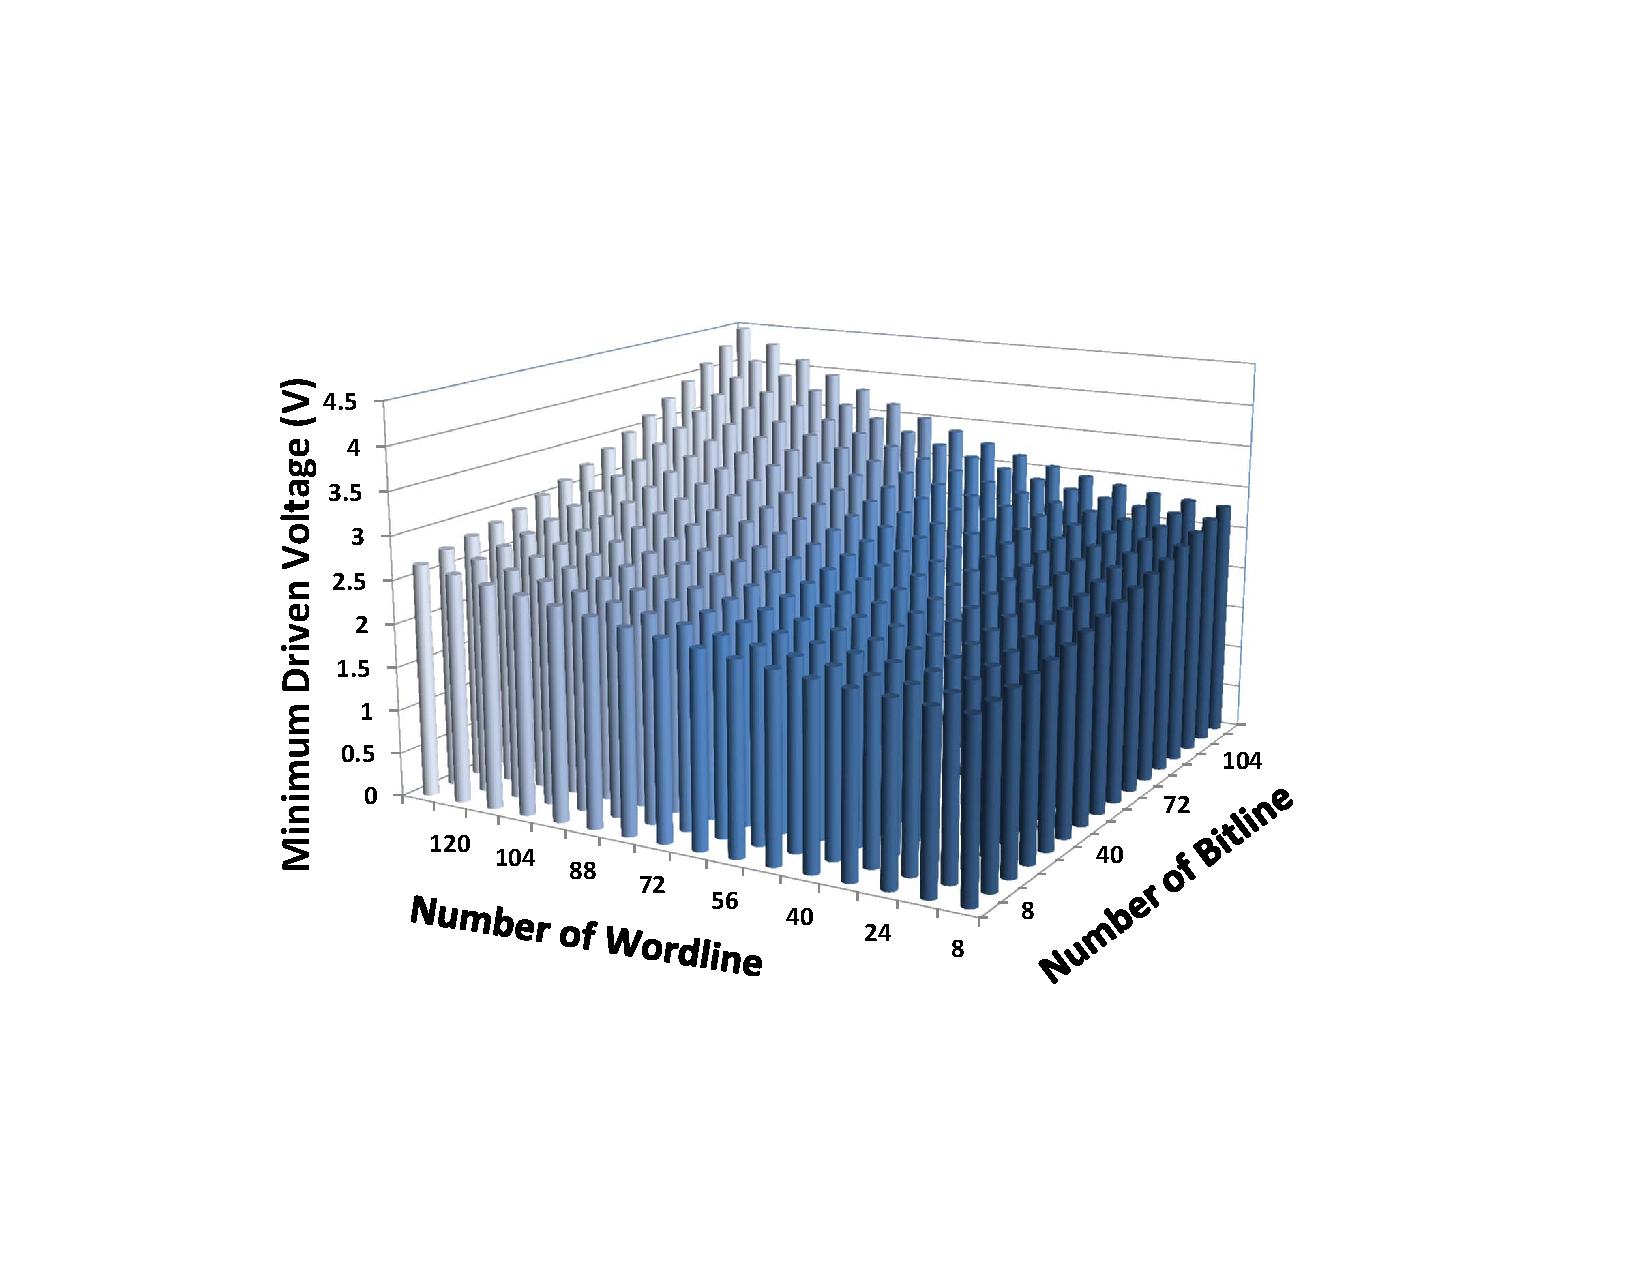
\includegraphics[width=0.45\textwidth]{./figures/worst_v_f.pdf}\\
  \caption{Write voltage requirement (Threshold voltage = 2V). }\label{fig:worst_v}
  \vspace{-5pt}
\end{figure}


\begin{figure}%[!t]
\centering
  % Requires \usepackage{graphicx}
  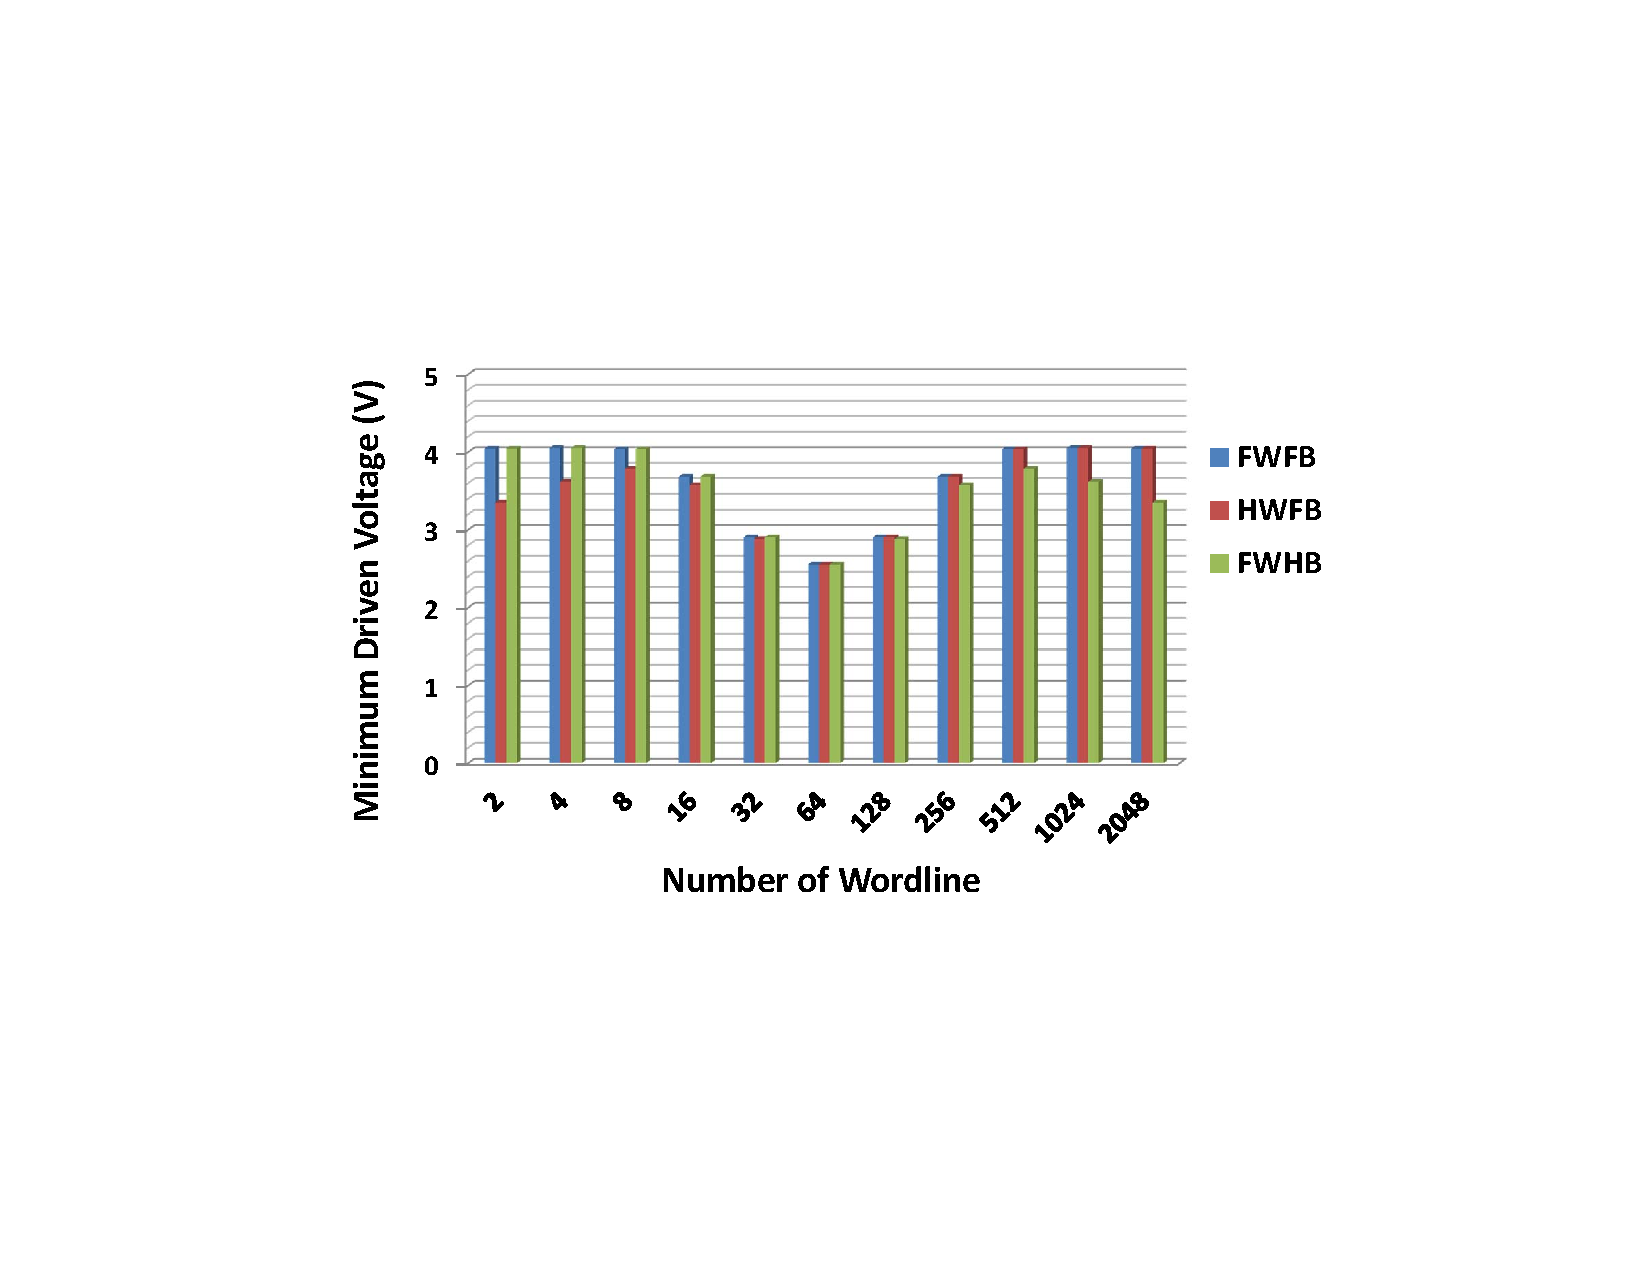
\includegraphics[width=0.45\textwidth]{./figures/shape_f.pdf}\\
  \caption{Write voltage requirement with different memory shape. (Array capacity = 256Kbits, Threshold voltage = 2V.)}\label{fig:shape}
    \vspace{-15pt}
\end{figure}

However, boosting the driven voltage also introduces other potential
problems for the array. In particular, increasing the driven voltage also
increases the voltage applied at unselected cells. Therefore, a write
disturbance may occur when the voltage applied at an unselected cell
exceeds the threshold voltage for SET or RESET operation. Specifically,
the maximum voltage applied at unselect cells is exactlly the same as half
of the driven voltage. Thus, only the array with driven voltage less than
4V are allowable.  Otherwise, the array is unreliable because it can not
avoid write failure and write disturbance at the same time. The unreliable
array sizes are denoted as red bars in Figure~\ref{fig:worst_v}. The array
size limitation provied by Figure~\ref{fig:worst_v} is a hard constraint
on array size, and all of the following energy and area tradeoffs should
be bounded by this constraint.


%Figure~\ref{fig:half} shows the maximum voltage applied at unselected
%cells with the minimum driven voltage, which is determined in
%Figure~\ref{fig:worst_v}. Since the threshold voltage of the ReRAM cell is
%2V, only array sizes with worst case unselected cell voltage less than 2V
%are allowable. Otherwise, the array is unreliable because it can not avoid
%write failure and write disturbance at the same time. Therefore,
%Figure~\ref{fig:half} provides a hard constraint on array size, and all of
%the following energy and area tradeoffs should be bounded by this
%constraint.

%\begin{figure}%[!t]
%\centering
%  % Requires \usepackage{graphicx}
%  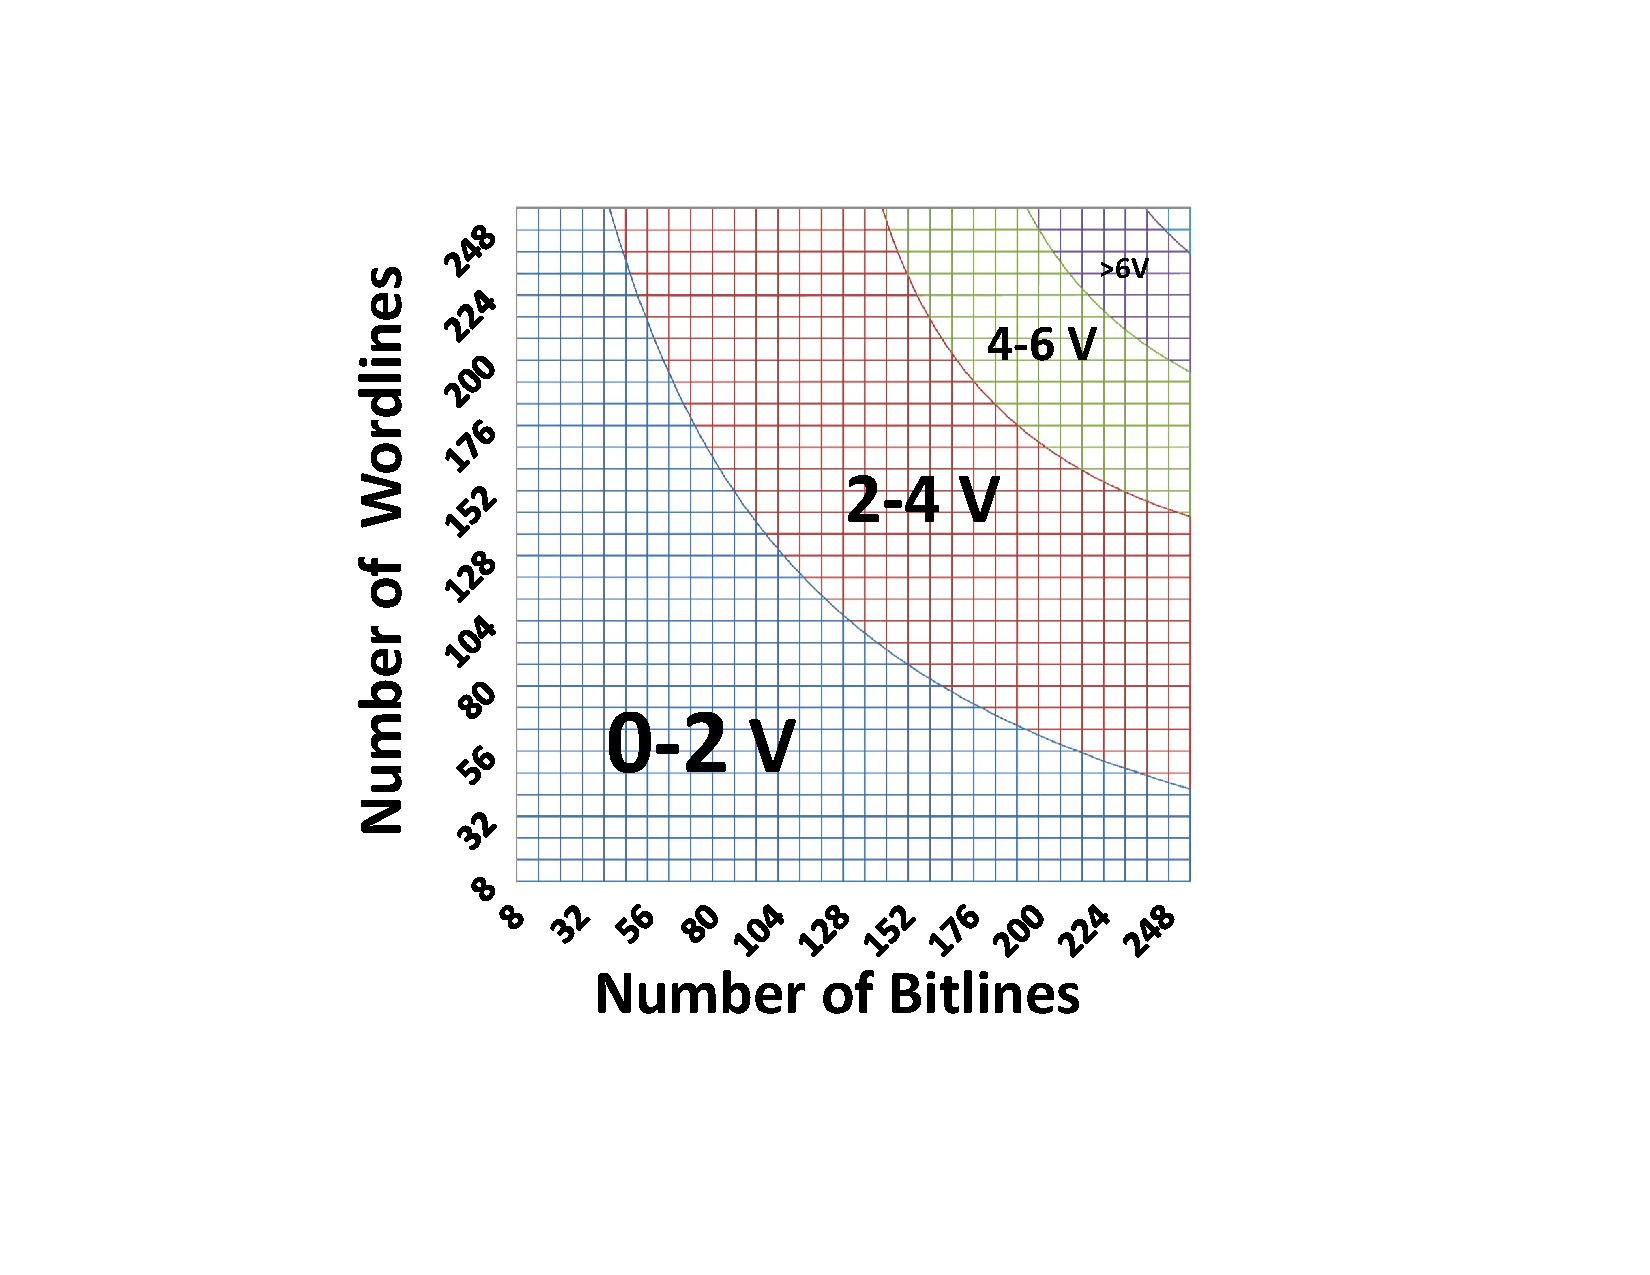
\includegraphics[width=0.28\textwidth]{./figures/Theoretical_bound_f.pdf}\\
%  \caption{The maximum voltage applied at unselected cells with the minimum driven voltage.}\label{fig:half}
%  \vspace{-10pt}
%\end{figure}


\vspace{6pt} \emph{Energy Consumption of Write Operation.} \vspace{6pt}

%The energy consumption of a write operation for a cross-point array can be calculated as:
%\begin{equation}
%E_{write} = E_{select} + E_{unselect} + E_{halfselect} + E_{line},
%\end{equation}
%where the $E_{select}$ is the energy consumed to change the state of the
%selected cell, the $E_{unselect}$ and $E_{halfselect}$ are the undesired
%energy wasted at the half selected and unselected cells. The energy
%consumed by the interconnect lines are represented by $E_{line}$.
%Figure~\ref{fig:energy} shows the decomposed energy consumption for the
%cross-point array. Note that, the $E_{line}$ and $E_{halfselect}$ take a
%large amount of the total energy consumption. Also, this part of energy
%wasted during the write operation takes greater part of the total energy
%for larger array sizes. For example, the undesired energy consumption for
%writing a $128{\times}128$ array is more than 1000 times larger than the
%$8{\times}8$ array. We also notice that, since the impact of sneak paths
%for floating schemes (FWHB and HWFB) is more serious, the energy consumed
%at unselected cells for floating schemes is larger than the half-biased
%scheme. Due to this reason, the total energy consumptions for FWHB and
%HWFB schemes are at least 10\% larger than that of HWHB scheme.
The energy consumption of a write operation includes: the energy consumed
to change the state of the selected cell (denoted as $E_{select}$), the
undesired energy wasted at the half selected cells ($E_{halfselect}$) and
unselected cells ($E_{unselect}$), as well as the energy consumed by the
interconnect lines ($E_{line}$). Figure~\ref{fig:energy}(a) shows the
decomposed energy consumption for the cross-point array. Note that, the
$E_{line}$ and $E_{halfselect}$ take a large amount of the total energy
consumption. Also, this part of energy wasted during the write operation
takes greater part of the total energy for larger array sizes. For
example, the undesired energy consumption for writing a $512{\times}512$
array is more than 15 times larger than that of a $32{\times}32$ array. We
also notice that, since the impact of sneak paths for floating schemes
(FWHB and HWFB) is more serious, the energy consumed at unselected cells
for floating schemes is larger than the half-biased scheme. Due to this
reason, the total energy consumptions for FWHB and HWFB schemes are at
least 10\% larger than that of HWHB scheme.

\begin{figure}%[!t]
\centering
  % Requires \usepackage{graphicx}
  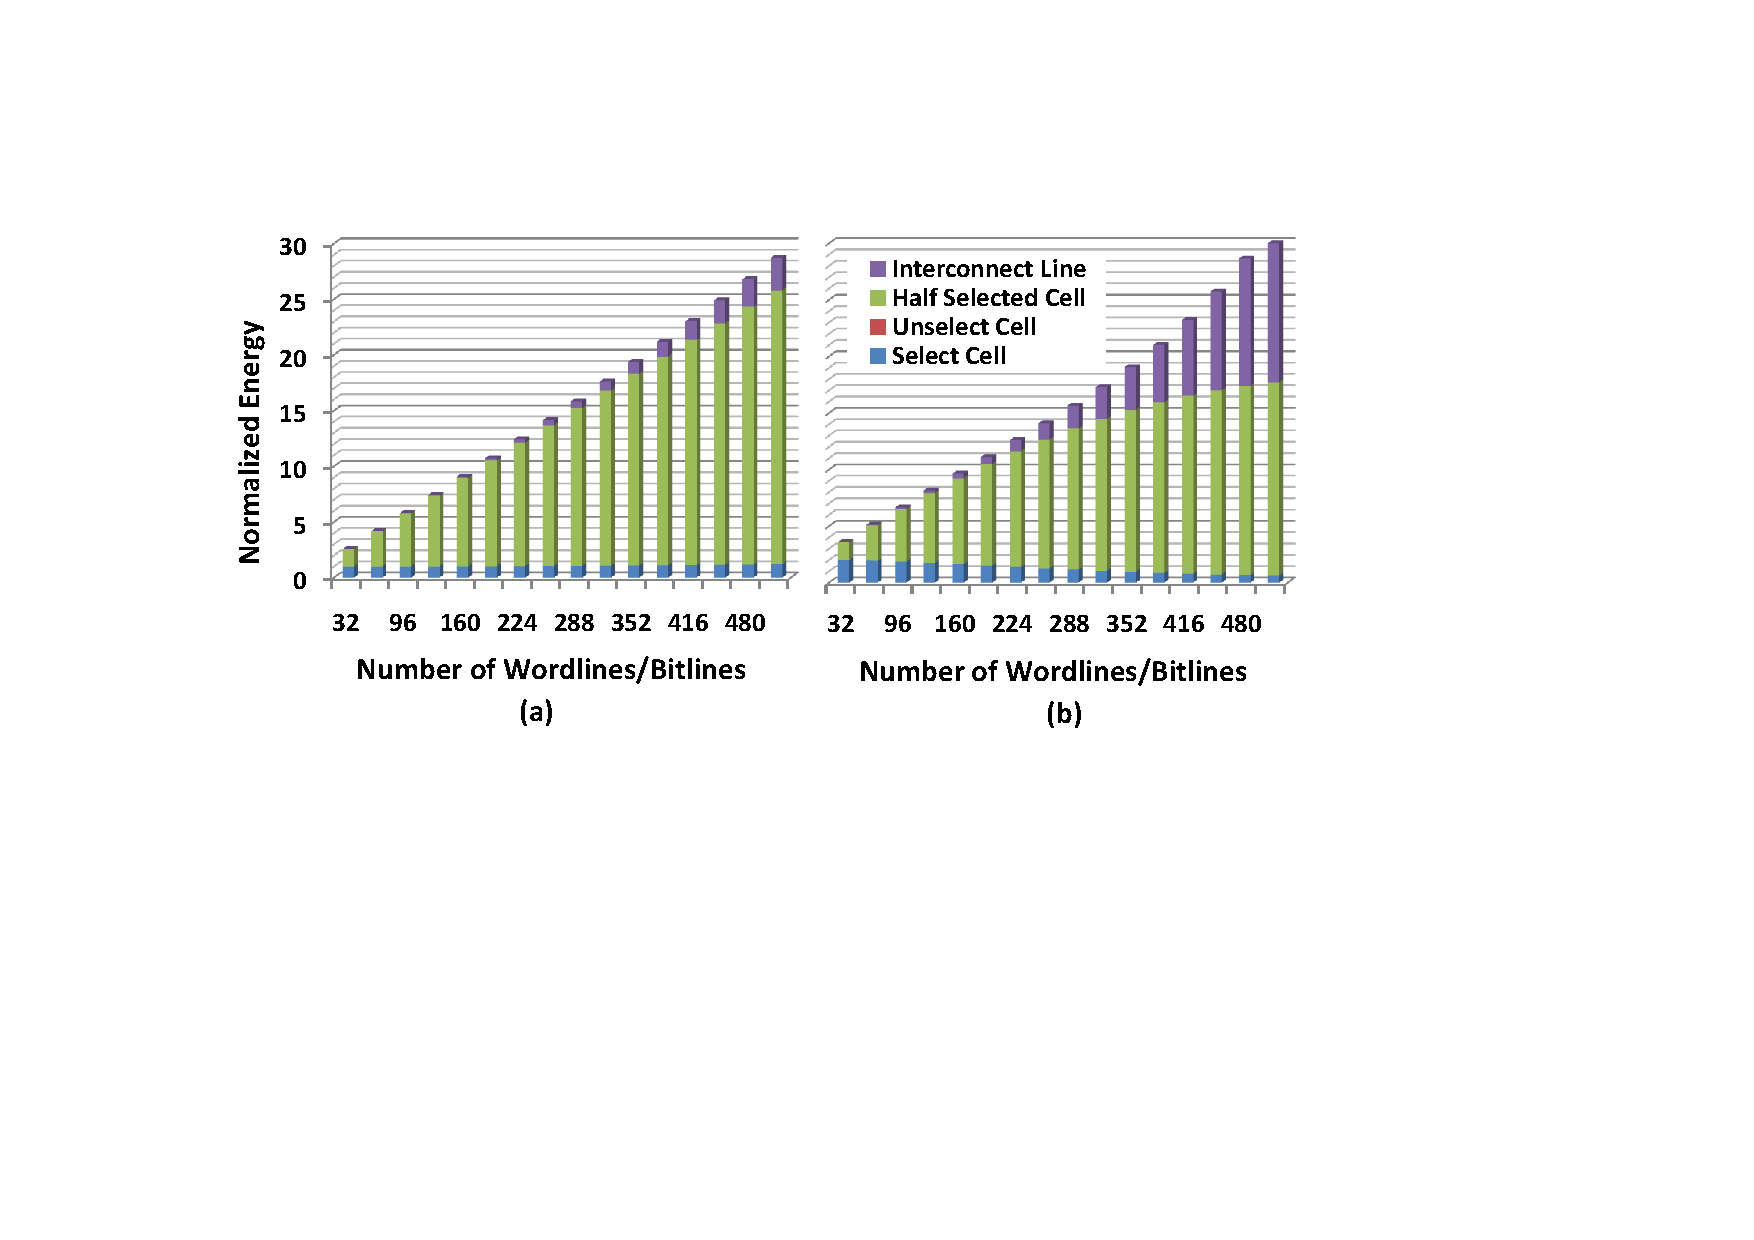
\includegraphics[width=0.5\textwidth]{./figures/energy_f_tall.pdf}\\
  \caption{The normalized energy consumption with different array size. (a): One bit writing; (b): Multi-bit writing.}\label{fig:energy}
    \vspace{-10pt}
\end{figure}

\vspace{6pt} \emph{Write Current and Area Overhead of Write Operation.}
\vspace{6pt}

The write operation for a $M \times N$ array requires $M$ wordline voltage
drivers and $N$ bitline multiplexers. The drivers and multiplexers should
be sized such that they can provide the worst-case current of wordline
current and bitline current. The transistor sizing of the wordline/bitline
circuitry are achieved using HSPICE simulations. We further calculate the
area overhead for the drivers and multiplexers by referring to the CACTI
area model. Figure~\ref{fig:drive_i}(a) shows the maximum write current
with different ReRAM array sizes. As we can see, the current requirement
increases slightly faster than linearly as array size increases. This is
primarily because we have to increase the write voltage to compensate the
voltage drop in large array size. Figure~\ref{fig:drive_i}(b) demonstrates
the area overhead for the wordline and bitline circuitry. It is indicated
that wordline drivers occupies comparable or even larger area than the
memory cells, degrading the effective cell size significantly. There are
two possible reasons: (1) wordline drivers are usually implemented as
tri-gates and larger than bitline multiplexers that are essentially pass
transistors; (2) wordline drivers have to provide more than one set of
write current in multi-bits write operation, as discussed in the following
section.

%\begin{figure}%[!t]
%\centering
%  % Requires \usepackage{graphicx}
%  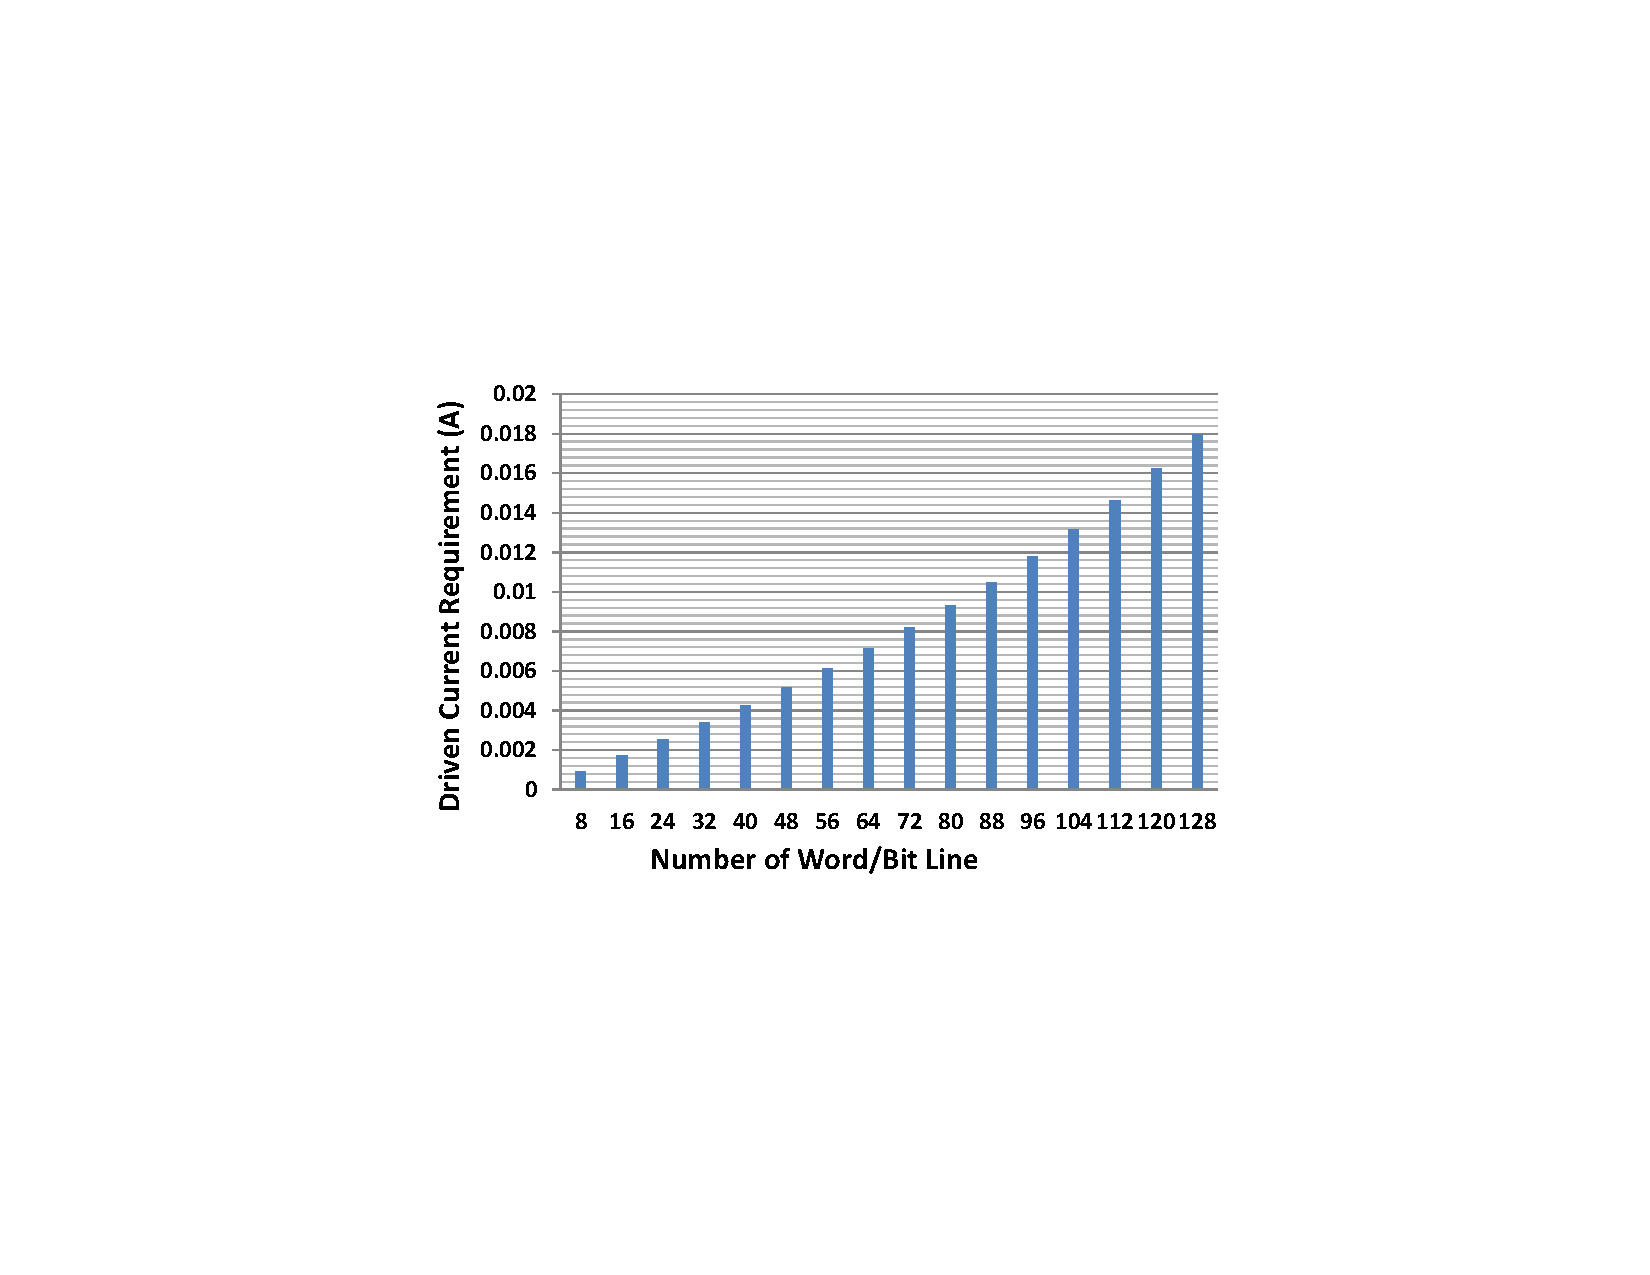
\includegraphics[width=0.4\textwidth]{./figures/w_current2.pdf}\\
%  \caption{The }\label{fig:w_current}
%\end{figure}
\begin{figure}%[!t]
\centering
  % Requires \usepackage{graphicx}
  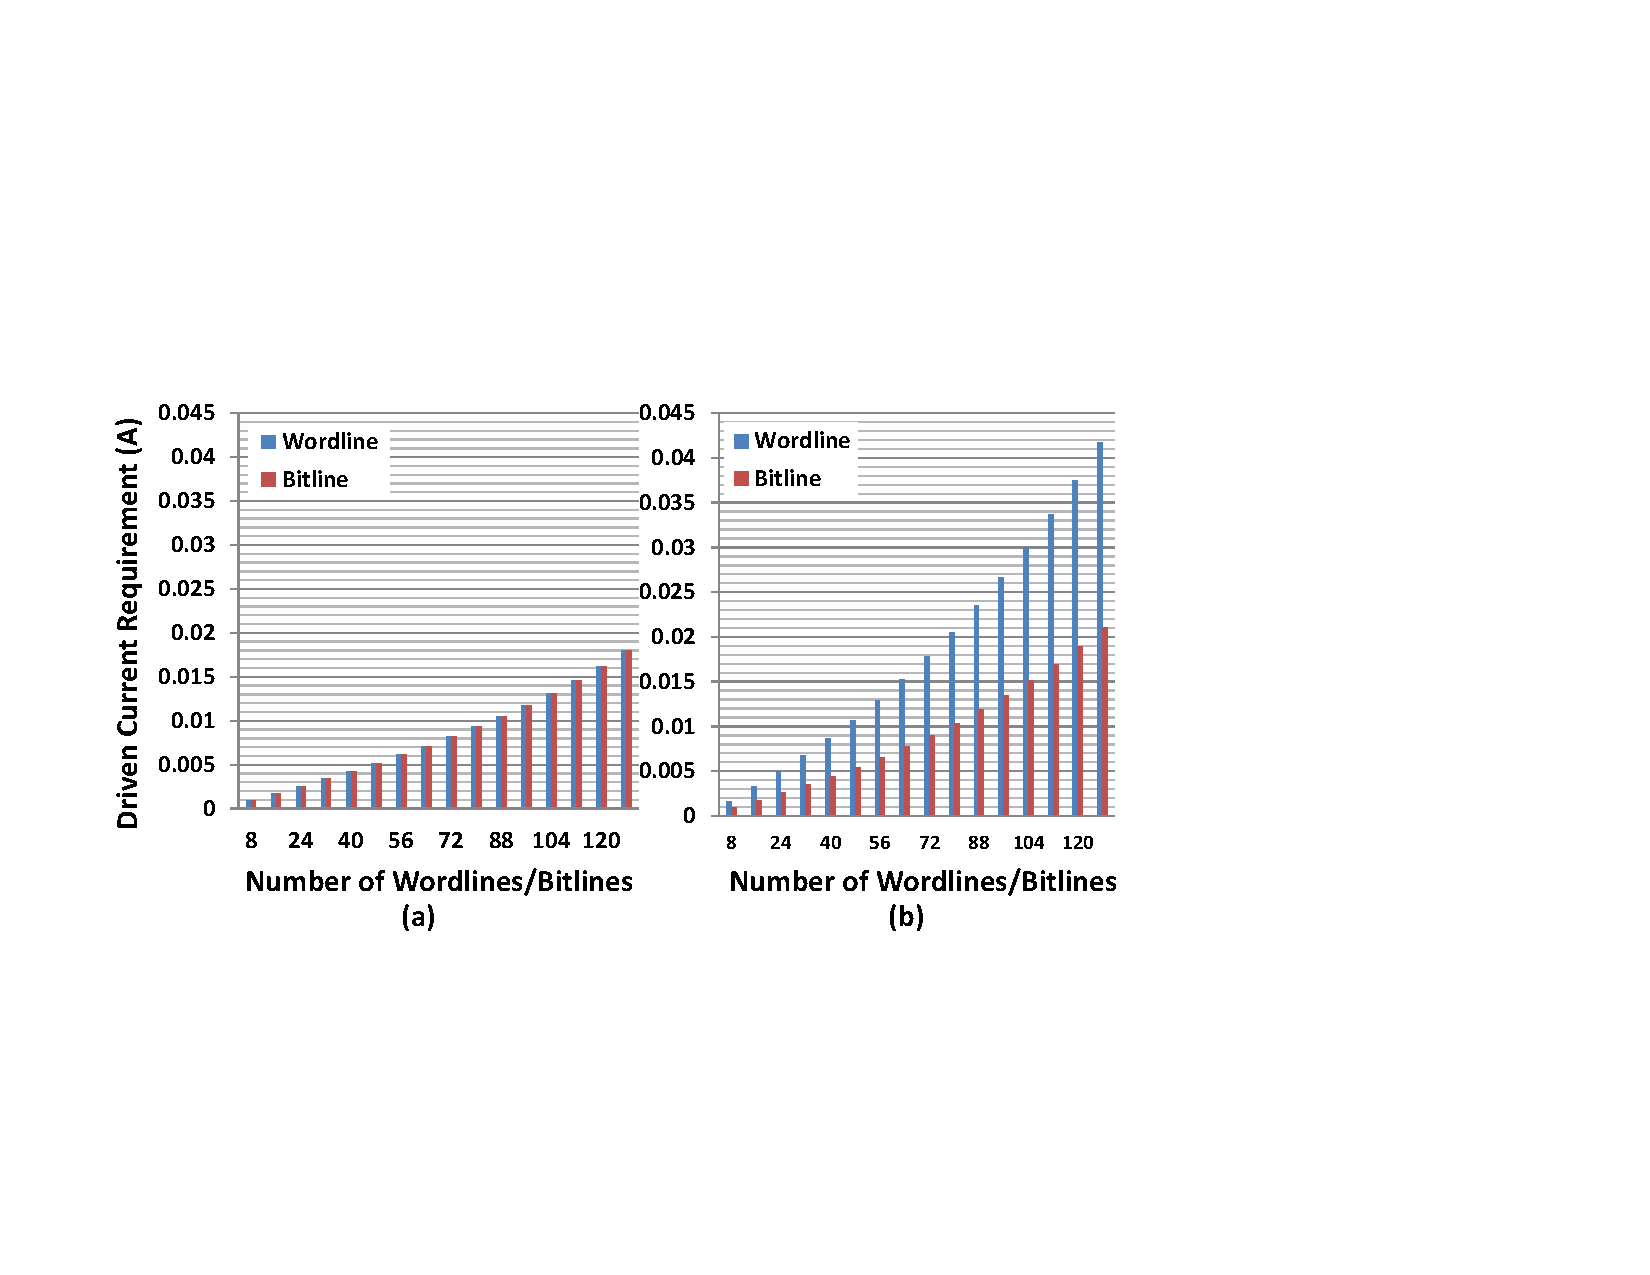
\includegraphics[width=0.5\textwidth]{./figures/drive_i_f.pdf}\\
  \caption{The driven current requirements for wordlines and bitlines. (a) One bit writing; (B) Multi-bit writing.}\label{fig:drive_i}
\end{figure}


\vspace{6pt} \emph{Discussion on Multi-Bits Write Operation.} \vspace{6pt}

So far, we have only discussed the write operation with one bit per
access. In this section, we consider the difference between one bit per
access and multi-bit per access write operations.

First of all, we evaluate the energy consumption of the write operation
that program one wordline at the same time. In order to fairly compare the
energy consumption, we compare the energy-per-bit instead of the total
energy. Besides, the multi-bit write operation required a two-step write
scheme. Therefore, in order to write a wordline with size of 512, the
energy-per-bit can be calculated as: $E_{ave}=E_{total}*2/512$.
Figure~\ref{fig:energy}(b) shows the energy-per-bit of the multi-bit write
operation. The energy shown in this figure is normalized to the same unit
as Figure~\ref{fig:energy}(a) for easier comparison. \textbf{The results
show that for large cross point array sizes, the multi-bit write operation
is much more energy efficient. This is because the energy wasted at the
unselected and half-selected cells are shared by multiple bits and the
average energy for one each bit is therefore reduced. However, although
the multi-bit write operation has the advantage of lower energy
consumption,} the maximum current requirement for each wordline also
increases. As shown in Figure~\ref{fig:drive_i}(b), the maximum driven
current for each bitline is almost the same as when writing one bit,
however the drive capability for each word line is >10 times larger than
that of  multi-bit writing. Since the area of the voltage driver increases
proportionally with its drive capability, the area overhead for multi-bit
writing is significantlly larger than for one bit writing. Due to the
space limitations, the results of area overhead are shown in the next
session.

%\begin{figure}%[!t]
%\centering
%  % Requires \usepackage{graphicx}
%  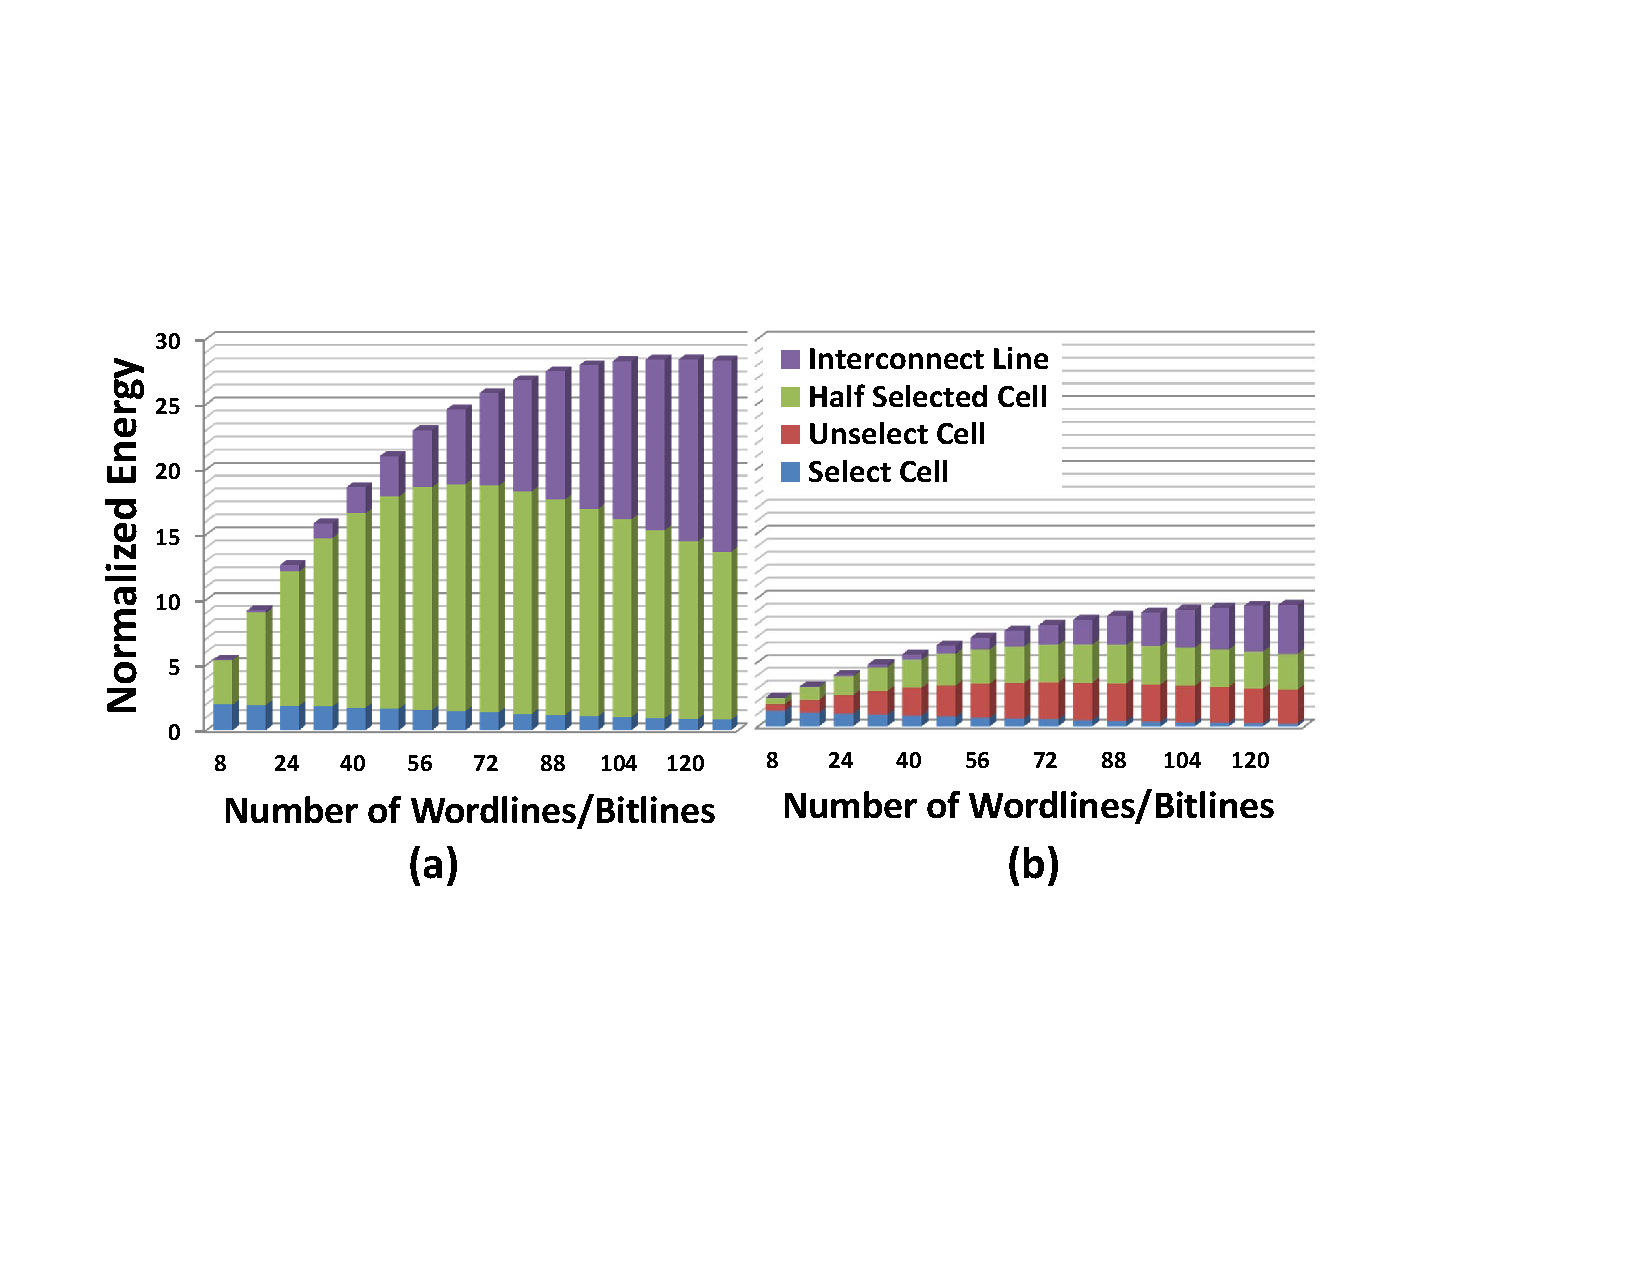
\includegraphics[width=0.5\textwidth]{./figures/multi_energy_f.pdf}\\
%  \caption{The normalized energy consumption per bit for multi-bits write operation. (a): HWHB and  FWHB schemes; (b): HWFB scheme. }\label{fig:multi_energy}
%    \vspace{-10pt}
%\end{figure}

In addition to the extra area overhead, writing multi-bit at a time will
also worsen the voltage drop along the wordline. As shown in
Figure~\ref{fig:multi_V}(a), in order to write a wordline per writing, the
reliable array size reduces to $352 \times 352$. \textbf{Compare to
Baseline and add discription for (b)}. 
%Therefore, as shown in Figure~\ref{fig:reliable_region},
%Therefore the simulation results show that the reliable size of the
%cross-point array will be further reduced. The maximum array size reduces
%from $116{\times}116$ to $100{\times}100$ for HWFB and HWFB schemes.
%For the energy consumption point of view, the one wordline write operation is more efficient.
\begin{figure}%[!t]
\centering
  % Requires \usepackage{graphicx}
  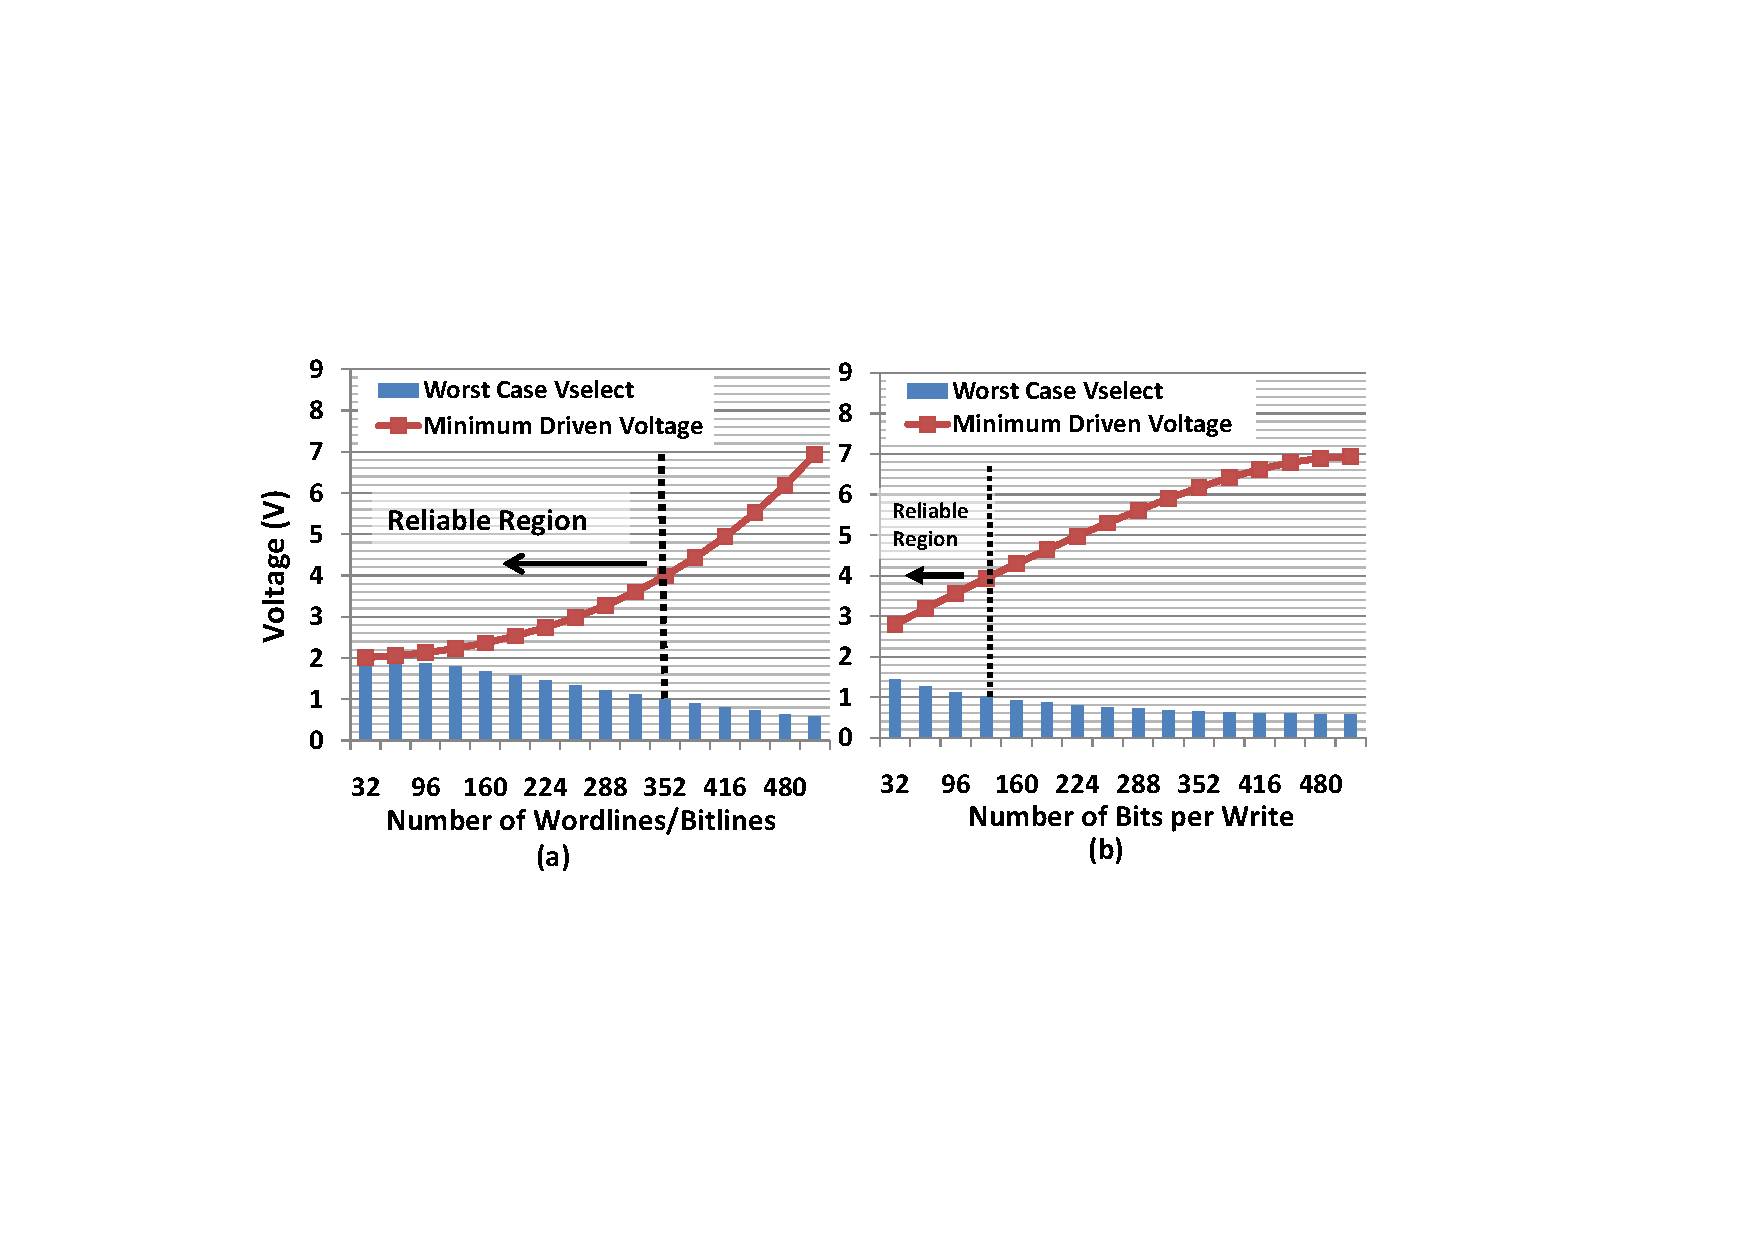
\includegraphics[width=0.5\textwidth]{./figures/multi_V.pdf}\label{fig:multi_V}\\
  \caption{Worst case voltage and write voltage requirment for multi-bit writing. (a) One wordline wrting with different array size; (b) 512x512 array with various number of bits per writing.}\label{fig:reliable_region}
    \vspace{-10pt}
\end{figure}
\subsection{Read Operation}
In this section we applied the similar sensing scheme as
\cite{crossbar_TED_2010} and \cite{crossbar_NANO08_Flocke}. In order to
read cell $R_{i,j}$, the $i^{th}$ wordline is biased at $V_{READ}$ and all
of the other wordlines and bitlines are grounded. Then the state of the
selected cell is read out by measuring the voltage across $R_s$. The
energy consumption for read operation can be analyzed by the same way as
that of the write operation. Since the read voltage is much smaller than
write voltage, the read energy is expected at least one order smaller than
write operation. Considerable sensing margin is achieved by implementing a
current-to-voltage converter and sensing the voltage signal using
traditional or emerging sense amplifier design. The input resistance of
the current-to-voltage converter is extracted from HSPICE simulation
results. Read sensing margin is defined as $\Delta V = \Delta I \times
R_{converter}$ where $R_{converter}$ is input resistance of the converter.

Additionally, since the read voltage/current is much lower than the write,
we believe that the voltage drivers can always provide enough current for
the read operation if they meet the current requirement for write
operation. Therefore, we can conclude that the area overhead of voltage
drivers is determined by the write current. However, the reliability of
read operation is different from the write operation. The read reliability
is determined by the voltage swing for reading HRS and LRS cells.
Figure~\ref{fig:sense_margin_basic} (a) shows the voltage swing with
different array sizes. Specifically, larger cross-point array have more
sneak paths, making the output voltage very sensitive to the data pattern
of unselected cell. Therefore, the sense marging decreases with the
increase of array size. In order to improve the reliability of the read
operation, a two-step sensing scheme can be applied, which senses the
current of an unselected cell first, then the overall current is sensed,
and after that the current difference is converted to the output voltage.
The voltage swing of this two-step sensing scheme is shown in
Figure~\ref{fig:sense_margin_basic} (b). By using this two-step sensing
schemes, the voltage swing for a given array size and non-linearity
coefficient is doubled.


%\begin{figure}%[!t]
%\centering
%  % Requires \usepackage{graphicx}
%  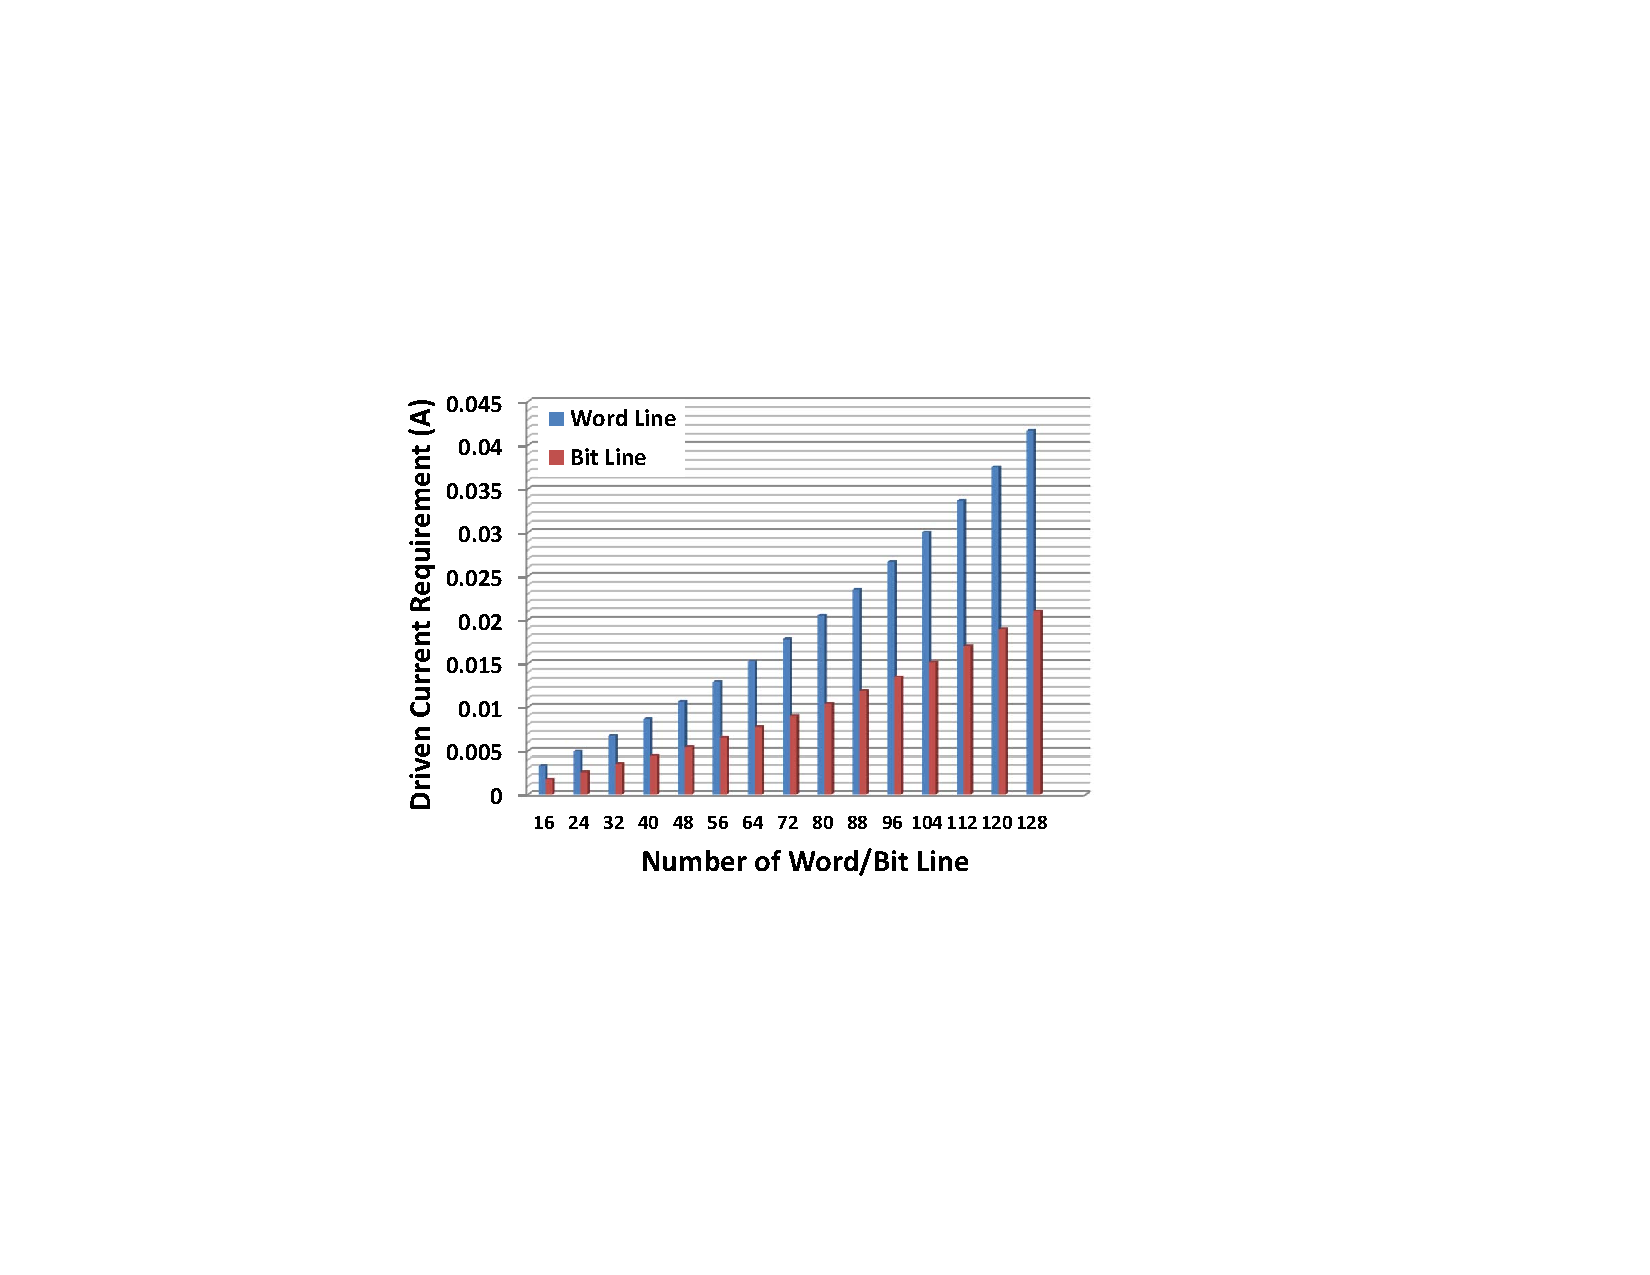
\includegraphics[width=0.4\textwidth]{./figures/multi_I2.pdf}\\
%  \caption{The }\label{fig:multi_I}
%\end{figure}


%\subsection{Read Operation}
%In this section we applied the similar sensing scheme as
%\cite{crossbar_TED_2010} and \cite{crossbar_NANO08_Flocke}. In order to
%read cell $R_{i,j}$, the $i^{th}$ wordline is biased at $V_{READ}$ and all
%of the other wordlines and bitlines are grounded. Then the state of the
%selected cell is read out by measuring the voltage across $R_s$. The
%energy consumption for read operation can be analyzed by the same way as
%that of the write operation. Since the read voltage is much smaller than
%write voltage, the read energy is expected at least one order smaller than
%write operation. Additionally, since the read voltage/current is much
%lower than the write, we believe that the voltage drivers can always
%provide enough current for the read operation if they meet the current
%requirement for write operation. Therefore, we can conclude that the area
%overhead of voltage drivers is determined by the write current. However,
%the reliability of read operation is different from the write operation.
%The read reliability is determined by the voltage swing for reading HRS
%and LRS cells. Figure~\ref{fig:sense_margin} (a) shows the voltage swing
%with different array sizes and $K_r$ values. Large array sizes and large
%non-linearity are harmful to the voltage swing: on the one hand, a larger
%array has more sneak paths, making the output voltage very sensitive to
%the data pattern of unselected cells; on the other hand, the non-linearity
%increases the resistance of LRS and therefore the resistance difference
%between HRS and LRS cells is reduced. In order to improve the reliability
%of the read operation, a two-step sensing scheme can be applied, which
%senses the current of an unselected cell first, then the overall current
%is sensed, and after that the current difference is converted to the
%output voltage. The voltage swing of this two-step sensing scheme is shown
%in Figure~\ref{fig:sense_margin} (b). By using this two-step sensing
%schemes, the voltage swing for a given array size and non-linearity
%coefficient is doubled.
%
%%\begin{figure}%[!t]
%%\centering
%%  % Requires \usepackage{graphicx}
%%  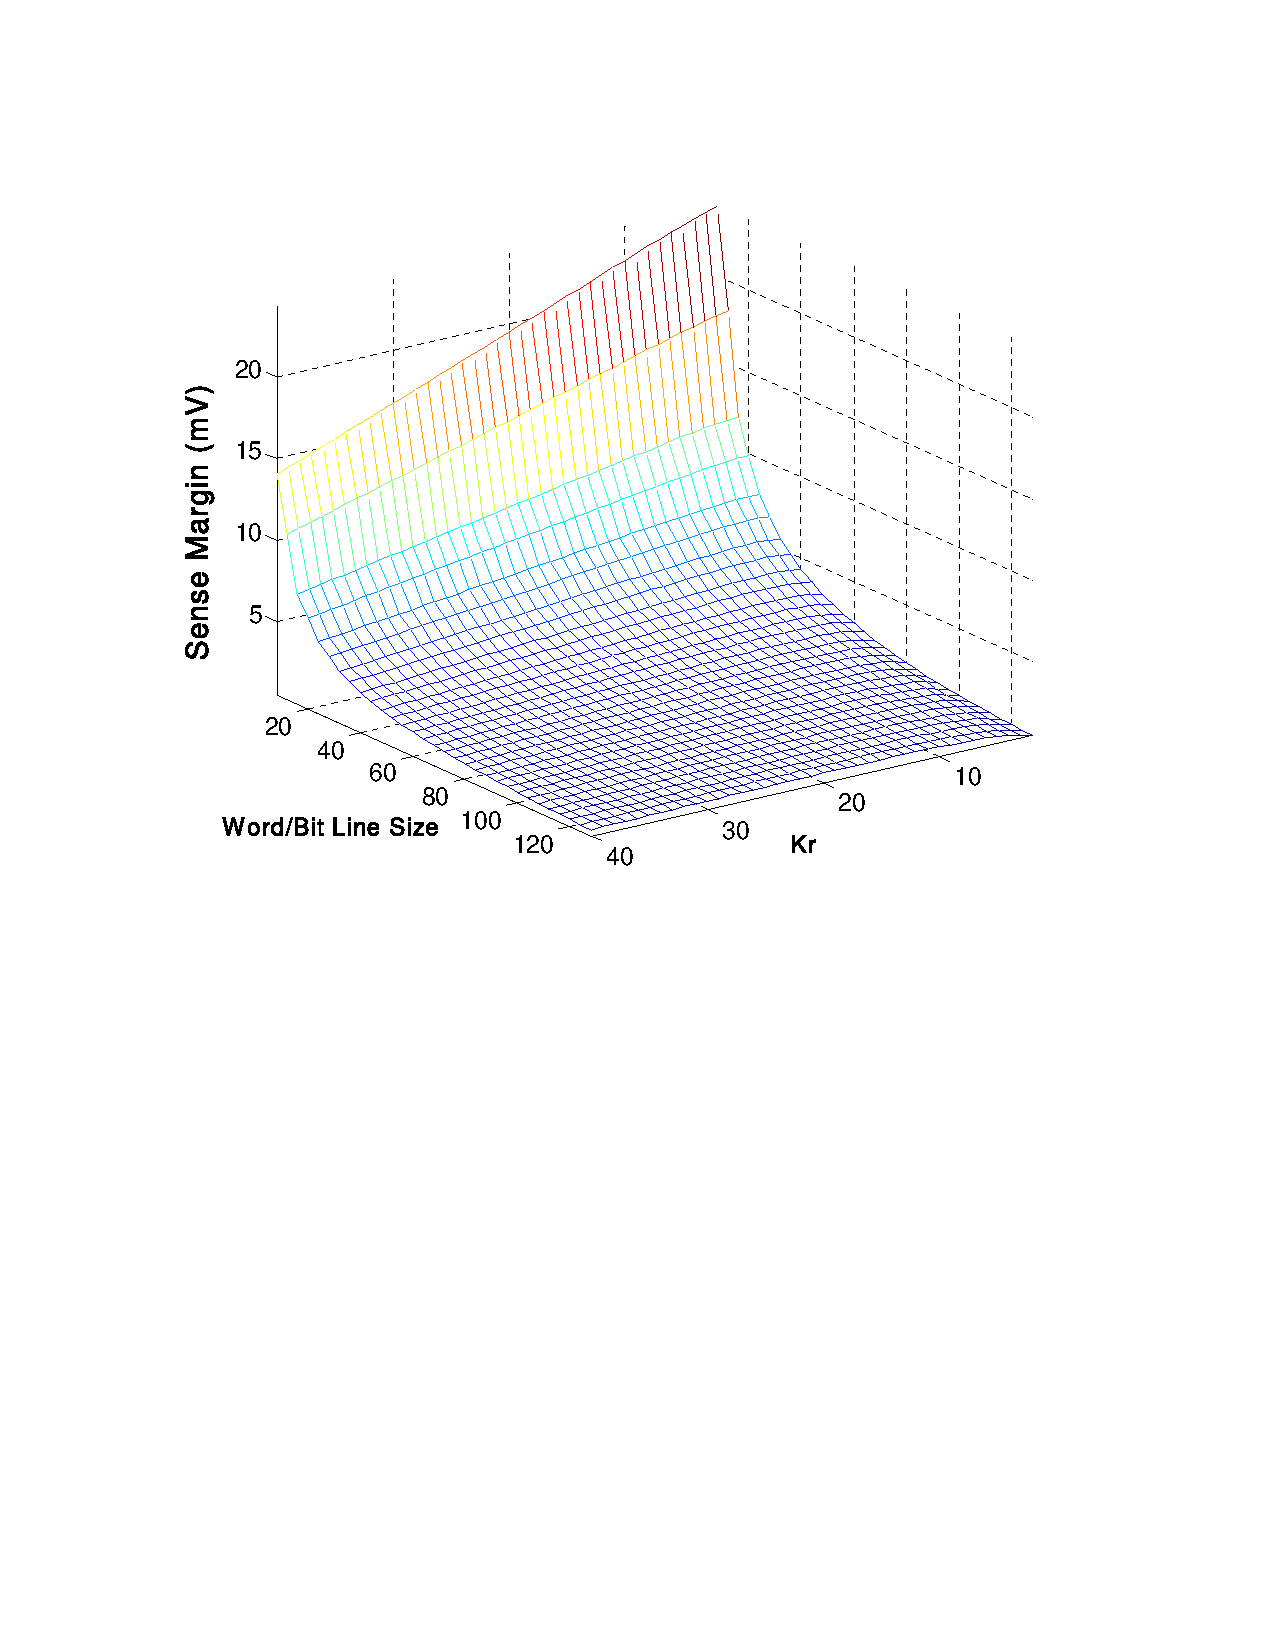
\includegraphics[width=0.45\textwidth]{./figures/margin.pdf}
%%  \caption{The}\label{fig:margin}
%%\end{figure}
%%
%%\begin{figure}%[!t]
%%\centering
%%  % Requires \usepackage{graphicx}
%%  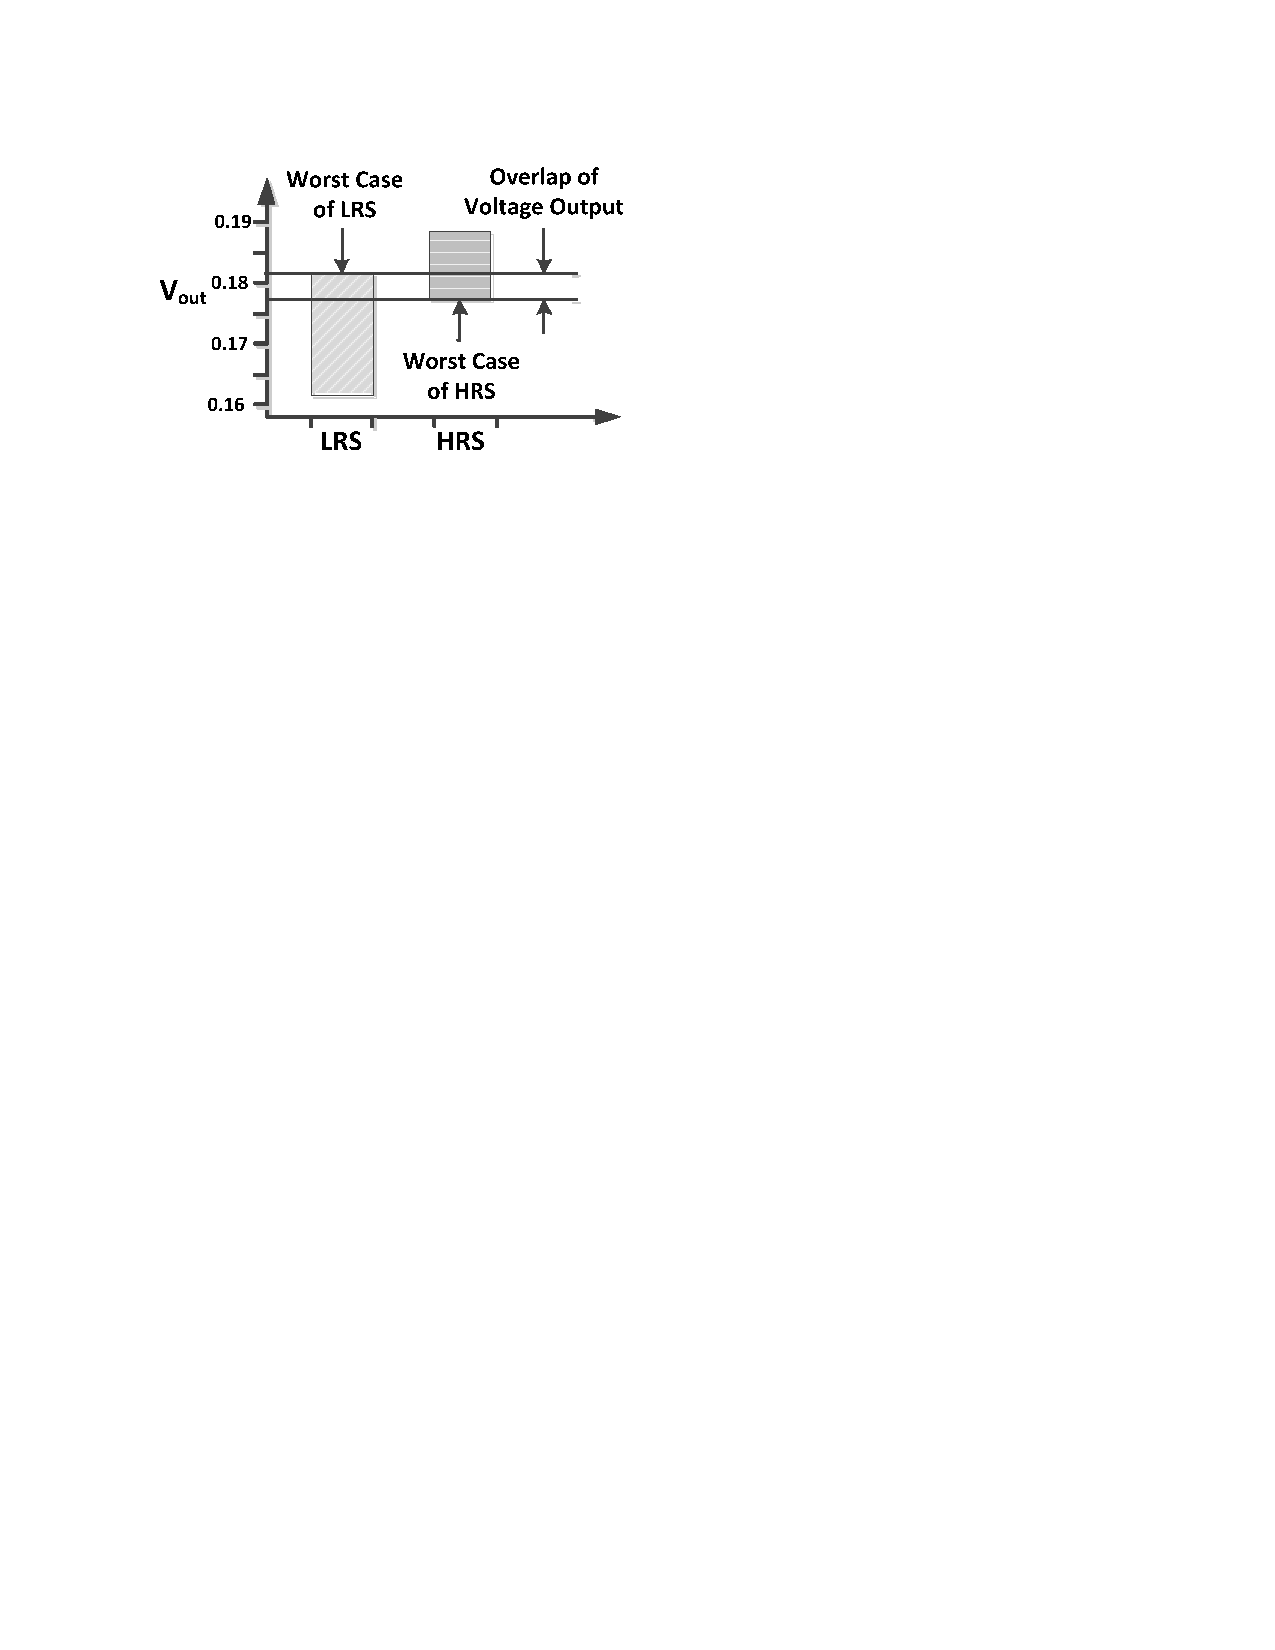
\includegraphics[width=0.4\textwidth]{./figures/overlap.pdf}\\
%%  \caption{The}\label{fig:overlap}
%%\end{figure}
%
%%
%%\begin{figure}%[!t]
%%\centering
%%  % Requires \usepackage{graphicx}
%%  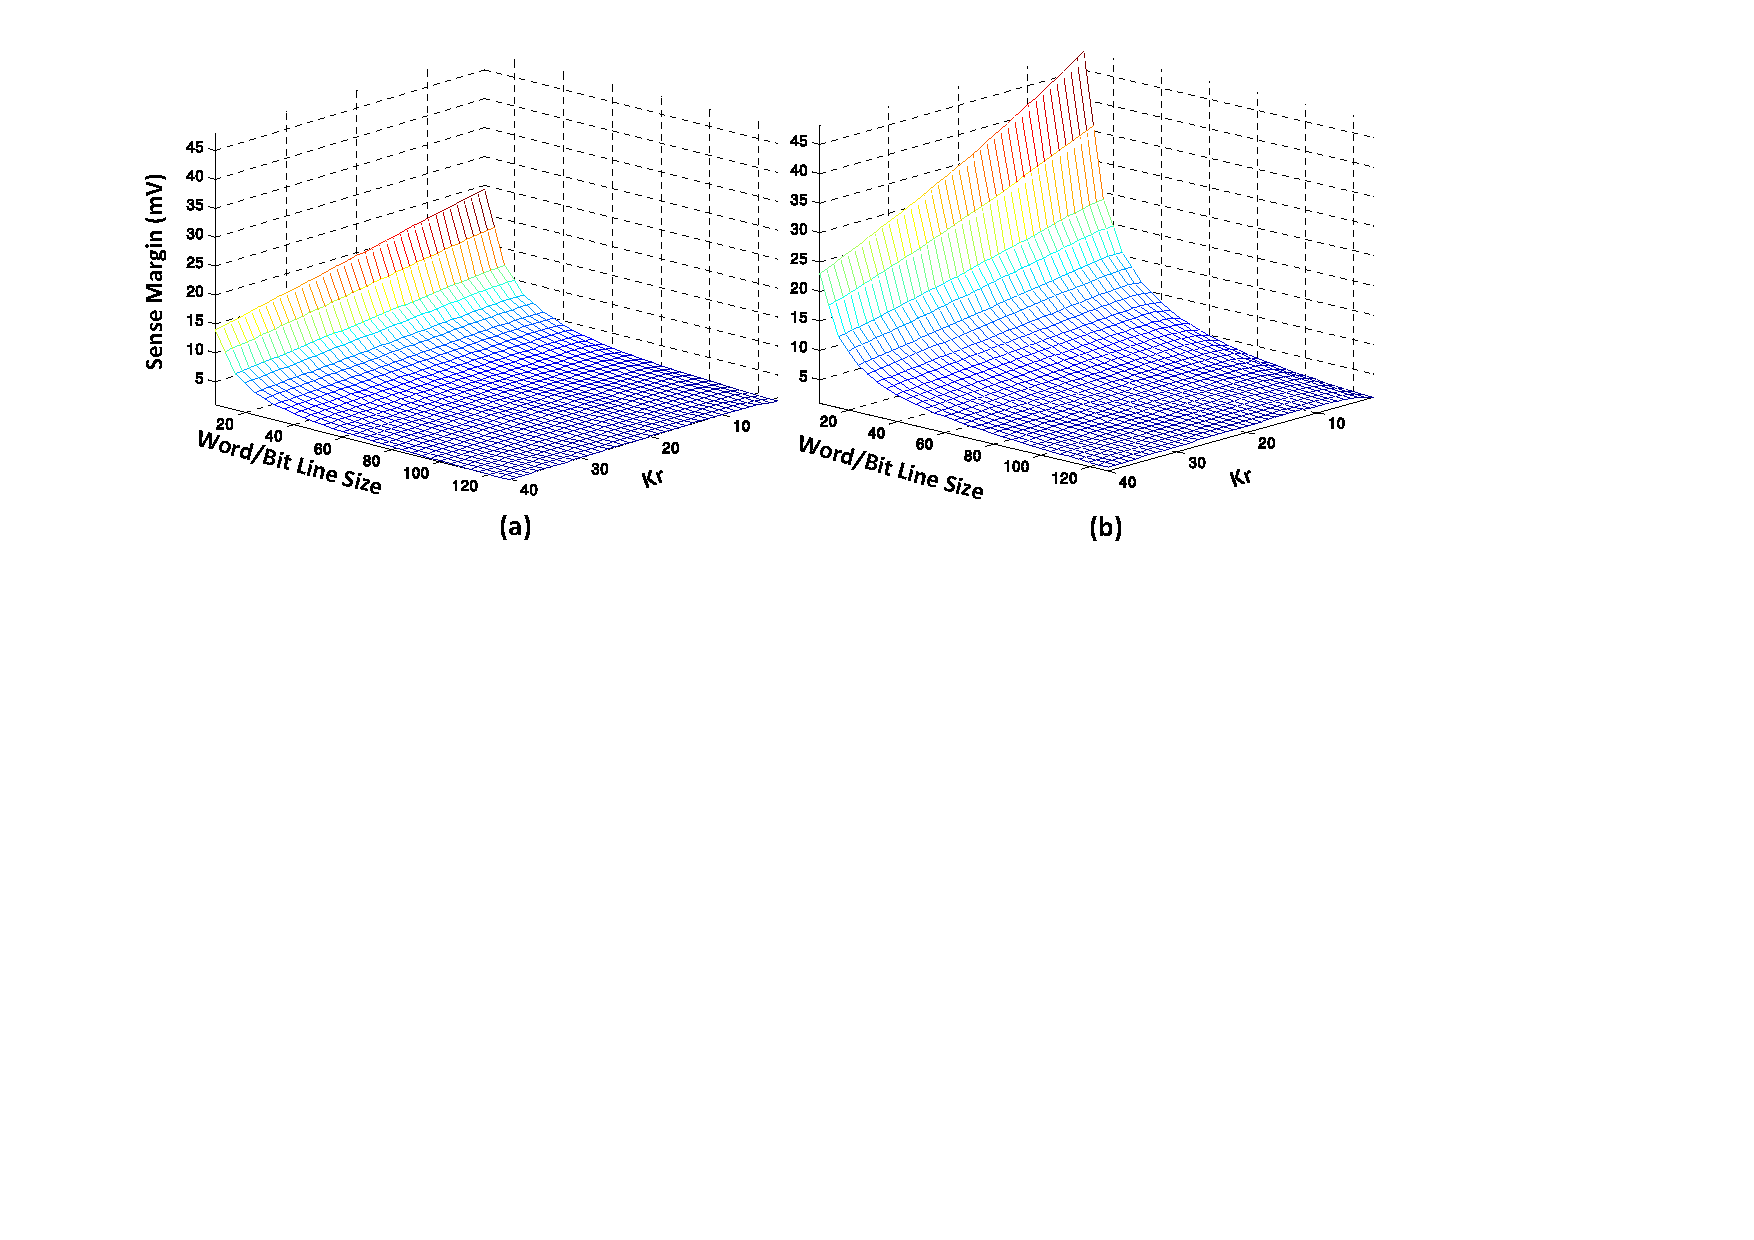
\includegraphics[width=0.5\textwidth]{./figures/sense_margin21}\\
%%  \caption{The}\label{fig:sense_margin}
%%\end{figure}
%
%\begin{figure}[!b]
%\centering
%  % Requires \usepackage{graphicx}
%  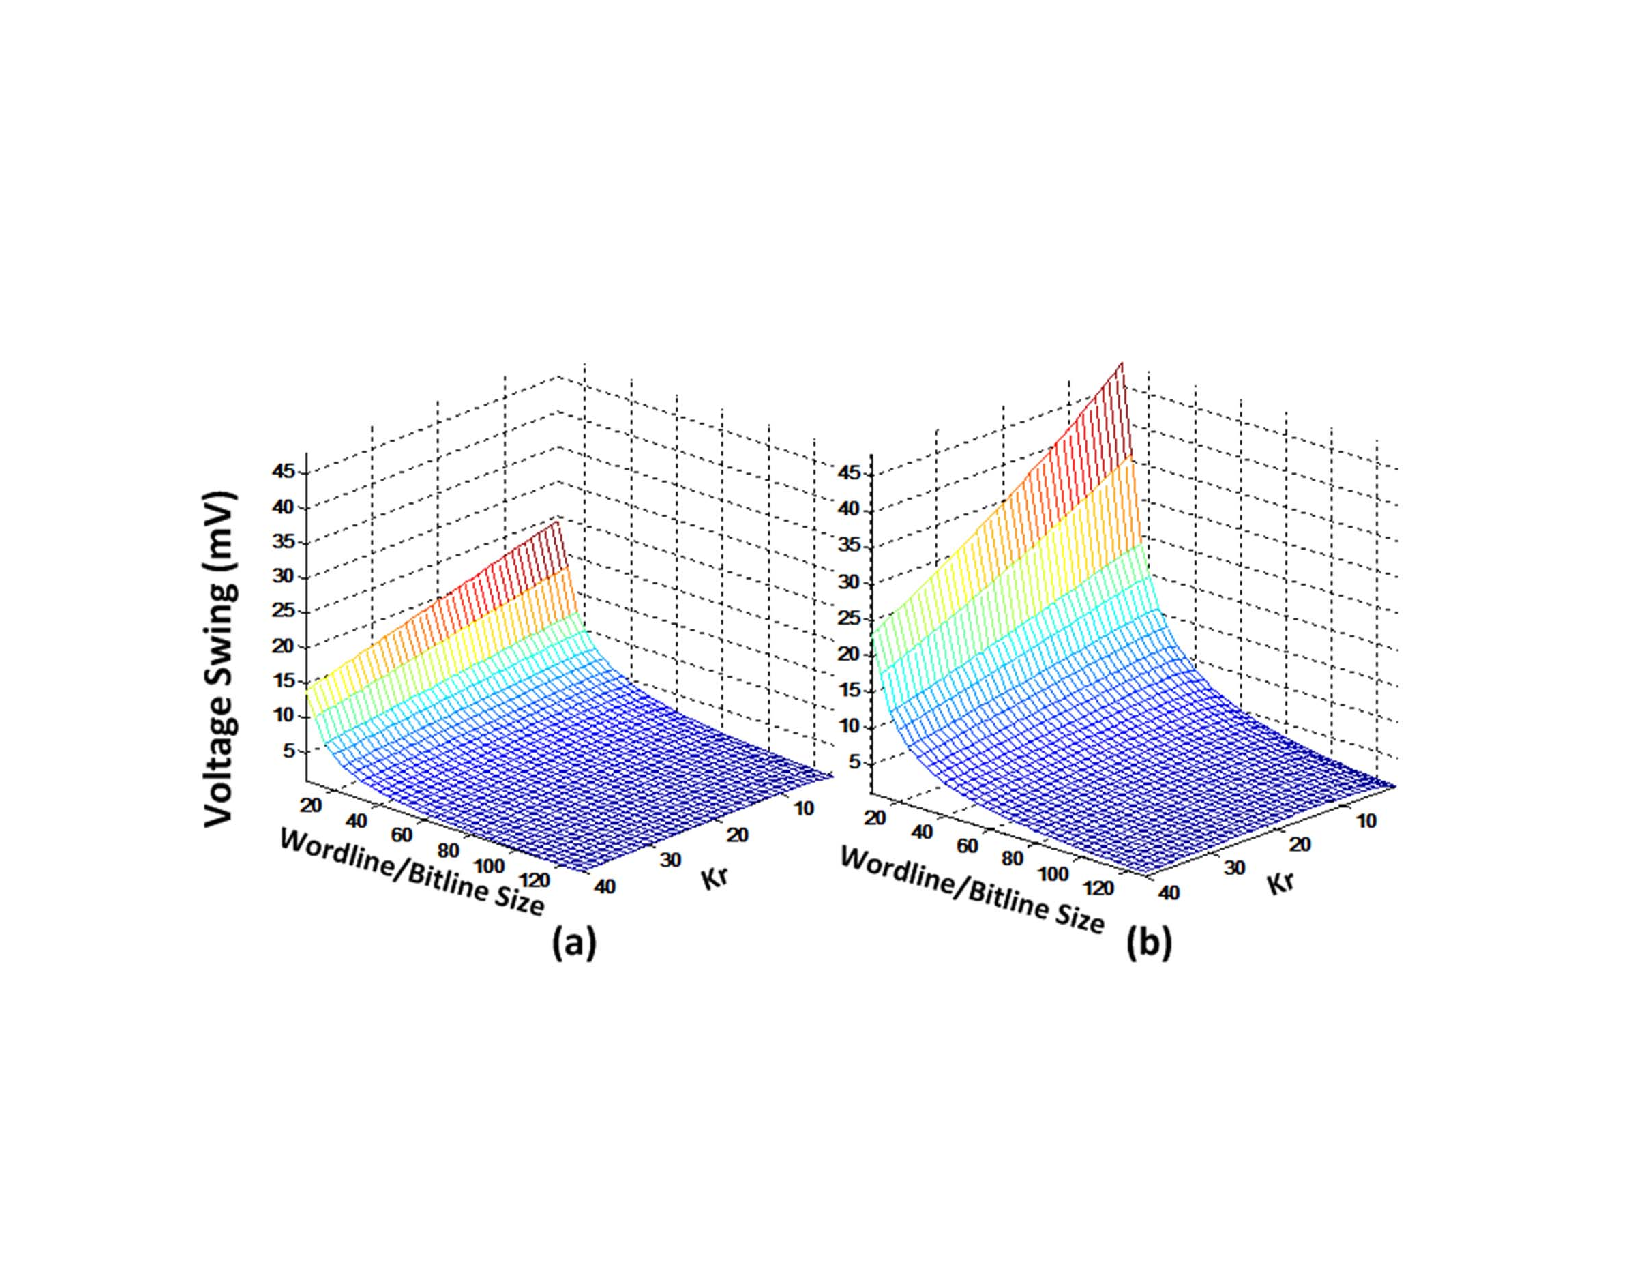
\includegraphics[width=0.5\textwidth]{./figures/sense_margin_f}\\
%  \caption{Relationships among the voltage swing, array size and non-linearity. (a) Normal sensing scheme; (b) Two-step sensing scheme}\label{fig:sense_margin}
%\end{figure}
